\documentclass[twoside]{article}

% Packages required by doxygen
\usepackage{calc}
\usepackage{doxygen}
\usepackage{graphicx}
\usepackage[utf8]{inputenc}
\usepackage{makeidx}
\usepackage{multicol}
\usepackage{multirow}
\usepackage{textcomp}
\usepackage[table]{xcolor}

% Font selection
\usepackage[T1]{fontenc}
\usepackage{mathptmx}
\usepackage[scaled=.90]{helvet}
\usepackage{courier}
\usepackage{amssymb}
\usepackage{sectsty}
\renewcommand{\familydefault}{\sfdefault}
\allsectionsfont{%
  \fontseries{bc}\selectfont%
  \color{darkgray}%
}
\renewcommand{\DoxyLabelFont}{%
  \fontseries{bc}\selectfont%
  \color{darkgray}%
}

% Page & text layout
\usepackage{geometry}
\geometry{%
  letterpaper,%
  top=2.5cm,%
  bottom=2.5cm,%
  left=2.5cm,%
  right=2.5cm%
}
\tolerance=750
\hfuzz=15pt
\hbadness=750
\setlength{\emergencystretch}{15pt}
\setlength{\parindent}{0cm}
\setlength{\parskip}{0.2cm}
\makeatletter
\renewcommand{\paragraph}{%
  \@startsection{paragraph}{4}{0ex}{-1.0ex}{1.0ex}{%
    \normalfont\normalsize\bfseries\SS@parafont%
  }%
}
\renewcommand{\subparagraph}{%
  \@startsection{subparagraph}{5}{0ex}{-1.0ex}{1.0ex}{%
    \normalfont\normalsize\bfseries\SS@subparafont%
  }%
}
\makeatother

% Headers & footers
\usepackage{fancyhdr}
\pagestyle{fancyplain}
\fancyhead[LE]{\fancyplain{}{\bfseries\thepage}}
\fancyhead[CE]{\fancyplain{}{}}
\fancyhead[RE]{\fancyplain{}{\bfseries\leftmark}}
\fancyhead[LO]{\fancyplain{}{\bfseries\rightmark}}
\fancyhead[CO]{\fancyplain{}{}}
\fancyhead[RO]{\fancyplain{}{\bfseries\thepage}}
\fancyfoot[LE]{\fancyplain{}{}}
\fancyfoot[CE]{\fancyplain{}{}}
\fancyfoot[RE]{\fancyplain{}{\bfseries\scriptsize Generated on Sun Jan 25 2015 10\-:31\-:51 for I\-M\-U\-Graph by Doxygen }}
\fancyfoot[LO]{\fancyplain{}{\bfseries\scriptsize Generated on Sun Jan 25 2015 10\-:31\-:51 for I\-M\-U\-Graph by Doxygen }}
\fancyfoot[CO]{\fancyplain{}{}}
\fancyfoot[RO]{\fancyplain{}{}}
\renewcommand{\footrulewidth}{0.4pt}
\renewcommand{\sectionmark}[1]{%
  \markright{\thesection\ #1}%
}

% Indices & bibliography
\usepackage{natbib}
\usepackage[titles]{tocloft}
\setcounter{tocdepth}{3}
\setcounter{secnumdepth}{5}
\makeindex

% Hyperlinks (required, but should be loaded last)
\usepackage{ifpdf}
\ifpdf
  \usepackage[pdftex,pagebackref=true]{hyperref}
\else
  \usepackage[ps2pdf,pagebackref=true]{hyperref}
\fi
\hypersetup{%
  colorlinks=true,%
  linkcolor=blue,%
  citecolor=blue,%
  unicode%
}

% Custom commands
\newcommand{\clearemptydoublepage}{%
  \newpage{\pagestyle{empty}\cleardoublepage}%
}


%===== C O N T E N T S =====

\begin{document}

% Titlepage & ToC
\hypersetup{pageanchor=false}
\pagenumbering{roman}
\begin{titlepage}
\vspace*{7cm}
\begin{center}%
{\Large I\-M\-U\-Graph }\\
\vspace*{1cm}
{\large Generated by Doxygen 1.8.6}\\
\vspace*{0.5cm}
{\small Sun Jan 25 2015 10:31:51}\\
\end{center}
\end{titlepage}
\tableofcontents
\pagenumbering{arabic}
\hypersetup{pageanchor=true}

%--- Begin generated contents ---
\section{I\-M\-U Graph}
\label{index}\hypertarget{index}{}\begin{DoxyAuthor}{Author}
Sebastián Sepúlveda 
\end{DoxyAuthor}
\begin{DoxyDate}{Date}
March 25, 2014 
\end{DoxyDate}
\begin{DoxyVersion}{Version}
0.\-9
\end{DoxyVersion}
\subsection*{Description}
\section{Todo List}
\label{todo}
\hypertarget{todo}{}

\begin{DoxyRefList}
\item[\label{todo__todo000001}%
\hypertarget{todo__todo000001}{}%
Class \hyperlink{classactivity_detection_1_1_activity_detection}{activity\-Detection.Activity\-Detection} ]Validate algorithms  
\item[\label{todo__todo000002}%
\hypertarget{todo__todo000002}{}%
Member \hyperlink{classactivity_detection_1_1_activity_detection_a25c0d2b32a72ac5be756a5fd74ee0c4c}{activity\-Detection.Activity\-Detection.update\-Activity} ]verify normalization of the I\-A\-A  
\item[\label{todo__todo000003}%
\hypertarget{todo__todo000003}{}%
Class \hyperlink{classfall_detection_1_1_fall_detection}{fall\-Detection.Fall\-Detection} ]Validate algorithms 
\end{DoxyRefList}
\section{Hierarchical Index}
\subsection{Class Hierarchy}
This inheritance list is sorted roughly, but not completely, alphabetically\-:\begin{DoxyCompactList}
\item \contentsline{section}{activity\-Detection.\-Activity\-Detection}{\pageref{classactivity_detection_1_1_activity_detection}}{}
\item \contentsline{section}{csv\-Export.\-C\-S\-V\-Export}{\pageref{classcsv_export_1_1_c_s_v_export}}{}
\item \contentsline{section}{fall\-Detection.\-Fall\-Detection}{\pageref{classfall_detection_1_1_fall_detection}}{}
\item \contentsline{section}{imu.\-I\-M\-U}{\pageref{classimu_1_1_i_m_u}}{}
\item \contentsline{section}{log.\-Log}{\pageref{classlog_1_1_log}}{}
\item object\begin{DoxyCompactList}
\item \contentsline{section}{gui.\-Ui\-\_\-\-Main\-Window}{\pageref{classgui_1_1_ui___main_window}}{}
\end{DoxyCompactList}
\item \contentsline{section}{posture.\-Posture}{\pageref{classposture_1_1_posture}}{}
\item Q\-Main\-Window\begin{DoxyCompactList}
\item \contentsline{section}{main.\-Main\-Window}{\pageref{classmain_1_1_main_window}}{}
\end{DoxyCompactList}
\item Q\-Thread\begin{DoxyCompactList}
\item \contentsline{section}{base\-Thread.\-Base\-Thread}{\pageref{classbase_thread_1_1_base_thread}}{}
\begin{DoxyCompactList}
\item \contentsline{section}{cube.\-Cube}{\pageref{classcube_1_1_cube}}{}
\item \contentsline{section}{serial\-Thread.\-Serial\-Thread}{\pageref{classserial_thread_1_1_serial_thread}}{}
\item \contentsline{section}{serial\-Thread\-\_\-mutiprocessing.\-Serial\-Thread}{\pageref{classserial_thread__mutiprocessing_1_1_serial_thread}}{}
\end{DoxyCompactList}
\end{DoxyCompactList}
\item \contentsline{section}{sensor\-Fusion.\-Sensor\-Fusion}{\pageref{classsensor_fusion_1_1_sensor_fusion}}{}
\end{DoxyCompactList}

\section{Class Index}
\subsection{Class List}
Here are the classes, structs, unions and interfaces with brief descriptions\-:\begin{DoxyCompactList}
\item\contentsline{section}{\hyperlink{classactivity_detection_1_1_activity_detection}{activity\-Detection.\-Activity\-Detection} \\*Estimates the energy consumption (Kcal) by second }{\pageref{classactivity_detection_1_1_activity_detection}}{}
\item\contentsline{section}{\hyperlink{classbase_thread_1_1_base_thread}{base\-Thread.\-Base\-Thread} \\*Defines basic methods for dealing with Qt Threads and all Threads }{\pageref{classbase_thread_1_1_base_thread}}{}
\item\contentsline{section}{\hyperlink{classcsv_export_1_1_c_s_v_export}{csv\-Export.\-C\-S\-V\-Export} \\*Export data in C\-S\-V format }{\pageref{classcsv_export_1_1_c_s_v_export}}{}
\item\contentsline{section}{\hyperlink{classcube_1_1_cube}{cube.\-Cube} \\*Displays the orientation as a 3\-D cube }{\pageref{classcube_1_1_cube}}{}
\item\contentsline{section}{\hyperlink{classfall_detection_1_1_fall_detection}{fall\-Detection.\-Fall\-Detection} \\*Detects fall from the accelerometer data }{\pageref{classfall_detection_1_1_fall_detection}}{}
\item\contentsline{section}{\hyperlink{classimu_1_1_i_m_u}{imu.\-I\-M\-U} \\*\hyperlink{classimu_1_1_i_m_u}{I\-M\-U} values for scales and data structure in the C\-S\-V data received }{\pageref{classimu_1_1_i_m_u}}{}
\item\contentsline{section}{\hyperlink{classlog_1_1_log}{log.\-Log} \\*General logging for debugging }{\pageref{classlog_1_1_log}}{}
\item\contentsline{section}{\hyperlink{classmain_1_1_main_window}{main.\-Main\-Window} \\*Managing and plotting adquired data }{\pageref{classmain_1_1_main_window}}{}
\item\contentsline{section}{\hyperlink{classposture_1_1_posture}{posture.\-Posture} \\*\hyperlink{classposture_1_1_posture}{Posture} estimation based on accelerometer used as a compensated tilt sensor }{\pageref{classposture_1_1_posture}}{}
\item\contentsline{section}{\hyperlink{classsensor_fusion_1_1_sensor_fusion}{sensor\-Fusion.\-Sensor\-Fusion} \\*Algorithms and functions for 9\-D\-O\-F fusion }{\pageref{classsensor_fusion_1_1_sensor_fusion}}{}
\item\contentsline{section}{\hyperlink{classserial_thread_1_1_serial_thread}{serial\-Thread.\-Serial\-Thread} \\*Obtain and scale serial data in a thread }{\pageref{classserial_thread_1_1_serial_thread}}{}
\item\contentsline{section}{\hyperlink{classserial_thread__mutiprocessing_1_1_serial_thread}{serial\-Thread\-\_\-mutiprocessing.\-Serial\-Thread} \\*Obtain and scale serial data in a thread }{\pageref{classserial_thread__mutiprocessing_1_1_serial_thread}}{}
\item\contentsline{section}{\hyperlink{classgui_1_1_ui___main_window}{gui.\-Ui\-\_\-\-Main\-Window} }{\pageref{classgui_1_1_ui___main_window}}{}
\end{DoxyCompactList}

\section{Class Documentation}
\hypertarget{classactivity_detection_1_1_activity_detection}{\subsection{activity\-Detection.\-Activity\-Detection Class Reference}
\label{classactivity_detection_1_1_activity_detection}\index{activity\-Detection.\-Activity\-Detection@{activity\-Detection.\-Activity\-Detection}}
}


Estimates the energy consumption (Kcal) by second.  


\subsubsection*{Public Member Functions}
\begin{DoxyCompactItemize}
\item 
def \hyperlink{classactivity_detection_1_1_activity_detection_a928cf245f832e26577625232d0803a47}{\-\_\-\-\_\-init\-\_\-\-\_\-}
\begin{DoxyCompactList}\small\item\em Constructor for Activity Detection. \end{DoxyCompactList}\item 
def \hyperlink{classactivity_detection_1_1_activity_detection_a65ceffc34852f2debf600096301d6217}{abs\-\_\-list}
\begin{DoxyCompactList}\small\item\em Take the absolute value of a list. \end{DoxyCompactList}\item 
def \hyperlink{classactivity_detection_1_1_activity_detection_a25c0d2b32a72ac5be756a5fd74ee0c4c}{update\-Activity}
\begin{DoxyCompactList}\small\item\em Update activity detection algorithm with last second data. \end{DoxyCompactList}\item 
def \hyperlink{classactivity_detection_1_1_activity_detection_aaedeb86760c2edb29274956e53240ecc}{get\-Energy\-Consumption}
\begin{DoxyCompactList}\small\item\em Getter for the last second energy consuption. \end{DoxyCompactList}\item 
def \hyperlink{classactivity_detection_1_1_activity_detection_a104e51a618c579e321f6a71f1e05cb87}{get\-E\-E}
\begin{DoxyCompactList}\small\item\em Getter for the E\-E value. \end{DoxyCompactList}\item 
def \hyperlink{classactivity_detection_1_1_activity_detection_a8dd2cc520a000ca555f8a478e11ffaf7}{get\-B\-M\-R}
\begin{DoxyCompactList}\small\item\em Getter for the B\-M\-R value. \end{DoxyCompactList}\end{DoxyCompactItemize}
\subsubsection*{Public Attributes}
\begin{DoxyCompactItemize}
\item 
\hypertarget{classactivity_detection_1_1_activity_detection_ac059a8775de7bbdd7e4e5d5d5bf8d238}{{\bfseries B\-M\-R}}\label{classactivity_detection_1_1_activity_detection_ac059a8775de7bbdd7e4e5d5d5bf8d238}

\item 
\hypertarget{classactivity_detection_1_1_activity_detection_a27126ac10d1900ab3eb87f4e0bfc1811}{{\bfseries fs}}\label{classactivity_detection_1_1_activity_detection_a27126ac10d1900ab3eb87f4e0bfc1811}

\item 
\hypertarget{classactivity_detection_1_1_activity_detection_a08d4f14a05d0a9c66e19463bdaa5c668}{{\bfseries E\-E}}\label{classactivity_detection_1_1_activity_detection_a08d4f14a05d0a9c66e19463bdaa5c668}

\end{DoxyCompactItemize}
\subsubsection*{Static Public Attributes}
\begin{DoxyCompactItemize}
\item 
int \hyperlink{classactivity_detection_1_1_activity_detection_a7a2350bfa80449984efa3e5ae313a29c}{B\-M\-R} = .\-023842593
\begin{DoxyCompactList}\small\item\em Default value for B\-M\-R. \end{DoxyCompactList}\item 
int \hyperlink{classactivity_detection_1_1_activity_detection_a1a2a17f907231e0ea52ab41de3aa54ed}{E\-E} = 0
\begin{DoxyCompactList}\small\item\em Predicted consumed energy by activity (E\-E) in a second. \end{DoxyCompactList}\item 
\hypertarget{classactivity_detection_1_1_activity_detection_a9480289ea33b66524afd3fc17c931bc8}{int {\bfseries fs} = .\-02}\label{classactivity_detection_1_1_activity_detection_a9480289ea33b66524afd3fc17c931bc8}

\end{DoxyCompactItemize}


\subsubsection{Detailed Description}
Estimates the energy consumption (Kcal) by second. 

Using an accelerometer and aditional data from the user calculates\-:
\begin{DoxyItemize}
\item Index of activity (I\-A\-A) in a second
\item Predicted consumed energy by activity (E\-E) in a second
\item Predicted consumed energy by basal metabolism (B\-M\-R) in a second
\end{DoxyItemize}

\begin{DoxyAuthor}{Author}
Dr. Pablo Reyes 

Sebastian Sepulveda 
\end{DoxyAuthor}
\begin{DoxyRefDesc}{Todo}
\item[\hyperlink{todo__todo000001}{Todo}]Validate algorithms \end{DoxyRefDesc}


\subsubsection{Constructor \& Destructor Documentation}
\hypertarget{classactivity_detection_1_1_activity_detection_a928cf245f832e26577625232d0803a47}{\index{activity\-Detection\-::\-Activity\-Detection@{activity\-Detection\-::\-Activity\-Detection}!\-\_\-\-\_\-init\-\_\-\-\_\-@{\-\_\-\-\_\-init\-\_\-\-\_\-}}
\index{\-\_\-\-\_\-init\-\_\-\-\_\-@{\-\_\-\-\_\-init\-\_\-\-\_\-}!activityDetection::ActivityDetection@{activity\-Detection\-::\-Activity\-Detection}}
\paragraph[{\-\_\-\-\_\-init\-\_\-\-\_\-}]{\setlength{\rightskip}{0pt plus 5cm}def activity\-Detection.\-Activity\-Detection.\-\_\-\-\_\-init\-\_\-\-\_\- (
\begin{DoxyParamCaption}
\item[{}]{self, }
\item[{}]{kg = {\ttfamily 70}, }
\item[{}]{cm = {\ttfamily 170}, }
\item[{}]{years = {\ttfamily 20}, }
\item[{}]{fs = {\ttfamily .02}}
\end{DoxyParamCaption}
)}}\label{classactivity_detection_1_1_activity_detection_a928cf245f832e26577625232d0803a47}


Constructor for Activity Detection. 

Initializes calculations for the user to determinate the B\-M\-R 
\begin{DoxyParams}{Parameters}
{\em self} & The object pointer \\
\hline
{\em kg} & Weight of the user, in Kg \\
\hline
{\em cm} & Height of the user, in cm \\
\hline
{\em years} & Years of the user \\
\hline
{\em fs} & Time between samples, in seconds \\
\hline
\end{DoxyParams}


\subsubsection{Member Function Documentation}
\hypertarget{classactivity_detection_1_1_activity_detection_a65ceffc34852f2debf600096301d6217}{\index{activity\-Detection\-::\-Activity\-Detection@{activity\-Detection\-::\-Activity\-Detection}!abs\-\_\-list@{abs\-\_\-list}}
\index{abs\-\_\-list@{abs\-\_\-list}!activityDetection::ActivityDetection@{activity\-Detection\-::\-Activity\-Detection}}
\paragraph[{abs\-\_\-list}]{\setlength{\rightskip}{0pt plus 5cm}def activity\-Detection.\-Activity\-Detection.\-abs\-\_\-list (
\begin{DoxyParamCaption}
\item[{}]{self, }
\item[{}]{\-\_\-list}
\end{DoxyParamCaption}
)}}\label{classactivity_detection_1_1_activity_detection_a65ceffc34852f2debf600096301d6217}


Take the absolute value of a list. 

In Python, the {\ttfamily abs} function can't return the absolute values from a list. This function is a workaround to this limitation. 
\begin{DoxyParams}{Parameters}
{\em self} & The object pointer \\
\hline
{\em \-\_\-list} & The original list to take the absolutes values \\
\hline
\end{DoxyParams}
\begin{DoxyReturn}{Returns}
The absolute values in the original list 
\end{DoxyReturn}
\hypertarget{classactivity_detection_1_1_activity_detection_a8dd2cc520a000ca555f8a478e11ffaf7}{\index{activity\-Detection\-::\-Activity\-Detection@{activity\-Detection\-::\-Activity\-Detection}!get\-B\-M\-R@{get\-B\-M\-R}}
\index{get\-B\-M\-R@{get\-B\-M\-R}!activityDetection::ActivityDetection@{activity\-Detection\-::\-Activity\-Detection}}
\paragraph[{get\-B\-M\-R}]{\setlength{\rightskip}{0pt plus 5cm}def activity\-Detection.\-Activity\-Detection.\-get\-B\-M\-R (
\begin{DoxyParamCaption}
\item[{}]{self}
\end{DoxyParamCaption}
)}}\label{classactivity_detection_1_1_activity_detection_a8dd2cc520a000ca555f8a478e11ffaf7}


Getter for the B\-M\-R value. 

Gets the calculated B\-M\-R for the user 
\begin{DoxyParams}{Parameters}
{\em self} & The object pointer \\
\hline
\end{DoxyParams}
\begin{DoxyReturn}{Returns}
Value of the B\-M\-R (per day) 
\end{DoxyReturn}
\hypertarget{classactivity_detection_1_1_activity_detection_a104e51a618c579e321f6a71f1e05cb87}{\index{activity\-Detection\-::\-Activity\-Detection@{activity\-Detection\-::\-Activity\-Detection}!get\-E\-E@{get\-E\-E}}
\index{get\-E\-E@{get\-E\-E}!activityDetection::ActivityDetection@{activity\-Detection\-::\-Activity\-Detection}}
\paragraph[{get\-E\-E}]{\setlength{\rightskip}{0pt plus 5cm}def activity\-Detection.\-Activity\-Detection.\-get\-E\-E (
\begin{DoxyParamCaption}
\item[{}]{self}
\end{DoxyParamCaption}
)}}\label{classactivity_detection_1_1_activity_detection_a104e51a618c579e321f6a71f1e05cb87}


Getter for the E\-E value. 

Gets the last E\-E result from the last \# \hyperlink{classactivity_detection_1_1_activity_detection_a25c0d2b32a72ac5be756a5fd74ee0c4c}{update\-Activity} call 
\begin{DoxyParams}{Parameters}
{\em self} & The object pointer \\
\hline
\end{DoxyParams}
\begin{DoxyReturn}{Returns}
Last second E\-E 
\end{DoxyReturn}
\hypertarget{classactivity_detection_1_1_activity_detection_aaedeb86760c2edb29274956e53240ecc}{\index{activity\-Detection\-::\-Activity\-Detection@{activity\-Detection\-::\-Activity\-Detection}!get\-Energy\-Consumption@{get\-Energy\-Consumption}}
\index{get\-Energy\-Consumption@{get\-Energy\-Consumption}!activityDetection::ActivityDetection@{activity\-Detection\-::\-Activity\-Detection}}
\paragraph[{get\-Energy\-Consumption}]{\setlength{\rightskip}{0pt plus 5cm}def activity\-Detection.\-Activity\-Detection.\-get\-Energy\-Consumption (
\begin{DoxyParamCaption}
\item[{}]{self}
\end{DoxyParamCaption}
)}}\label{classactivity_detection_1_1_activity_detection_aaedeb86760c2edb29274956e53240ecc}


Getter for the last second energy consuption. 

Gets the last energy consumption result from the last \hyperlink{classactivity_detection_1_1_activity_detection_a25c0d2b32a72ac5be756a5fd74ee0c4c}{update\-Activity} call 
\begin{DoxyParams}{Parameters}
{\em self} & The object pointer \\
\hline
\end{DoxyParams}
\begin{DoxyReturn}{Returns}
Last second energy consumption, in Calories 
\end{DoxyReturn}
\hypertarget{classactivity_detection_1_1_activity_detection_a25c0d2b32a72ac5be756a5fd74ee0c4c}{\index{activity\-Detection\-::\-Activity\-Detection@{activity\-Detection\-::\-Activity\-Detection}!update\-Activity@{update\-Activity}}
\index{update\-Activity@{update\-Activity}!activityDetection::ActivityDetection@{activity\-Detection\-::\-Activity\-Detection}}
\paragraph[{update\-Activity}]{\setlength{\rightskip}{0pt plus 5cm}def activity\-Detection.\-Activity\-Detection.\-update\-Activity (
\begin{DoxyParamCaption}
\item[{}]{self, }
\item[{}]{x, }
\item[{}]{y, }
\item[{}]{z}
\end{DoxyParamCaption}
)}}\label{classactivity_detection_1_1_activity_detection_a25c0d2b32a72ac5be756a5fd74ee0c4c}


Update activity detection algorithm with last second data. 

The function updates the I\-A\-A based on the provided accelerations and calculates the energy consuptiom (E\-E). Updates the data for the algoritm 
\begin{DoxyParams}{Parameters}
{\em self} & The object pointer \\
\hline
{\em x} & list with the last second acceleration data in the X axis \\
\hline
{\em y} & list with the last second acceleration data in the Y axis \\
\hline
{\em z} & list with the last second acceleration data in the Z axis \\
\hline
\end{DoxyParams}
\begin{DoxyRefDesc}{Todo}
\item[\hyperlink{todo__todo000002}{Todo}]verify normalization of the I\-A\-A \end{DoxyRefDesc}


\subsubsection{Member Data Documentation}
\hypertarget{classactivity_detection_1_1_activity_detection_a7a2350bfa80449984efa3e5ae313a29c}{\index{activity\-Detection\-::\-Activity\-Detection@{activity\-Detection\-::\-Activity\-Detection}!B\-M\-R@{B\-M\-R}}
\index{B\-M\-R@{B\-M\-R}!activityDetection::ActivityDetection@{activity\-Detection\-::\-Activity\-Detection}}
\paragraph[{B\-M\-R}]{\setlength{\rightskip}{0pt plus 5cm}int activity\-Detection.\-Activity\-Detection.\-B\-M\-R = .\-023842593\hspace{0.3cm}{\ttfamily [static]}}}\label{classactivity_detection_1_1_activity_detection_a7a2350bfa80449984efa3e5ae313a29c}


Default value for B\-M\-R. 

Default B\-M\-R calculated at 2060 Kcal (normal person) divided in the seconds of one day (86400 seconds) \hypertarget{classactivity_detection_1_1_activity_detection_a1a2a17f907231e0ea52ab41de3aa54ed}{\index{activity\-Detection\-::\-Activity\-Detection@{activity\-Detection\-::\-Activity\-Detection}!E\-E@{E\-E}}
\index{E\-E@{E\-E}!activityDetection::ActivityDetection@{activity\-Detection\-::\-Activity\-Detection}}
\paragraph[{E\-E}]{\setlength{\rightskip}{0pt plus 5cm}int activity\-Detection.\-Activity\-Detection.\-E\-E = 0\hspace{0.3cm}{\ttfamily [static]}}}\label{classactivity_detection_1_1_activity_detection_a1a2a17f907231e0ea52ab41de3aa54ed}


Predicted consumed energy by activity (E\-E) in a second. 

Initalized at 0 

The documentation for this class was generated from the following file\-:\begin{DoxyCompactItemize}
\item 
I\-M\-U\-Graph/activity\-Detection.\-py\end{DoxyCompactItemize}

\hypertarget{classbase_thread_1_1_base_thread}{\subsection{base\-Thread.\-Base\-Thread Class Reference}
\label{classbase_thread_1_1_base_thread}\index{base\-Thread.\-Base\-Thread@{base\-Thread.\-Base\-Thread}}
}


Defines basic methods for dealing with Qt Threads and all Threads.  




Inheritance diagram for base\-Thread.\-Base\-Thread\-:\nopagebreak
\begin{figure}[H]
\begin{center}
\leavevmode
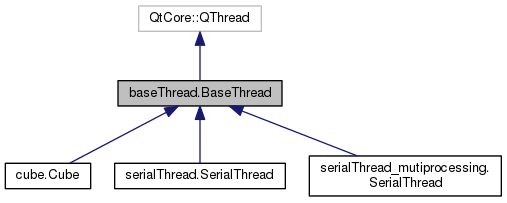
\includegraphics[width=350pt]{classbase_thread_1_1_base_thread__inherit__graph}
\end{center}
\end{figure}


Collaboration diagram for base\-Thread.\-Base\-Thread\-:\nopagebreak
\begin{figure}[H]
\begin{center}
\leavevmode
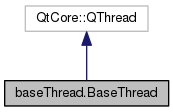
\includegraphics[width=202pt]{classbase_thread_1_1_base_thread__coll__graph}
\end{center}
\end{figure}
\subsubsection*{Public Member Functions}
\begin{DoxyCompactItemize}
\item 
def \hyperlink{classbase_thread_1_1_base_thread_a822975cc7b8816f501bfd1b71f6256b3}{\-\_\-\-\_\-init\-\_\-\-\_\-}
\begin{DoxyCompactList}\small\item\em Constructor. \end{DoxyCompactList}\item 
def \hyperlink{classbase_thread_1_1_base_thread_a5c6a3cad56112212c8106a205d0be359}{\-\_\-\-\_\-del\-\_\-\-\_\-}
\begin{DoxyCompactList}\small\item\em Deconstructor. \end{DoxyCompactList}\end{DoxyCompactItemize}
\subsubsection*{Public Attributes}
\begin{DoxyCompactItemize}
\item 
\hypertarget{classbase_thread_1_1_base_thread_af914ab68bce2b84935aa1b8246173114}{\hyperlink{classbase_thread_1_1_base_thread_af914ab68bce2b84935aa1b8246173114}{exiting}}\label{classbase_thread_1_1_base_thread_af914ab68bce2b84935aa1b8246173114}

\begin{DoxyCompactList}\small\item\em Notifies all threads to stop. \end{DoxyCompactList}\end{DoxyCompactItemize}


\subsubsection{Detailed Description}
Defines basic methods for dealing with Qt Threads and all Threads. 

Implement handles for the events of the Qt Threads and U\-I elements (main thread and U\-I thread). 

\subsubsection{Constructor \& Destructor Documentation}
\hypertarget{classbase_thread_1_1_base_thread_a822975cc7b8816f501bfd1b71f6256b3}{\index{base\-Thread\-::\-Base\-Thread@{base\-Thread\-::\-Base\-Thread}!\-\_\-\-\_\-init\-\_\-\-\_\-@{\-\_\-\-\_\-init\-\_\-\-\_\-}}
\index{\-\_\-\-\_\-init\-\_\-\-\_\-@{\-\_\-\-\_\-init\-\_\-\-\_\-}!baseThread::BaseThread@{base\-Thread\-::\-Base\-Thread}}
\paragraph[{\-\_\-\-\_\-init\-\_\-\-\_\-}]{\setlength{\rightskip}{0pt plus 5cm}def base\-Thread.\-Base\-Thread.\-\_\-\-\_\-init\-\_\-\-\_\- (
\begin{DoxyParamCaption}
\item[{}]{self}
\end{DoxyParamCaption}
)}}\label{classbase_thread_1_1_base_thread_a822975cc7b8816f501bfd1b71f6256b3}


Constructor. 

Initializes threads 
\begin{DoxyParams}{Parameters}
{\em self} & The objetc pointer \\
\hline
\end{DoxyParams}
\hypertarget{classbase_thread_1_1_base_thread_a5c6a3cad56112212c8106a205d0be359}{\index{base\-Thread\-::\-Base\-Thread@{base\-Thread\-::\-Base\-Thread}!\-\_\-\-\_\-del\-\_\-\-\_\-@{\-\_\-\-\_\-del\-\_\-\-\_\-}}
\index{\-\_\-\-\_\-del\-\_\-\-\_\-@{\-\_\-\-\_\-del\-\_\-\-\_\-}!baseThread::BaseThread@{base\-Thread\-::\-Base\-Thread}}
\paragraph[{\-\_\-\-\_\-del\-\_\-\-\_\-}]{\setlength{\rightskip}{0pt plus 5cm}def base\-Thread.\-Base\-Thread.\-\_\-\-\_\-del\-\_\-\-\_\- (
\begin{DoxyParamCaption}
\item[{}]{self}
\end{DoxyParamCaption}
)}}\label{classbase_thread_1_1_base_thread_a5c6a3cad56112212c8106a205d0be359}


Deconstructor. 

Closes and exits from threads 
\begin{DoxyParams}{Parameters}
{\em self} & The objetc pointer \\
\hline
\end{DoxyParams}


The documentation for this class was generated from the following file\-:\begin{DoxyCompactItemize}
\item 
I\-M\-U\-Graph/base\-Thread.\-py\end{DoxyCompactItemize}

\hypertarget{classcsv_export_1_1_c_s_v_export}{\subsection{csv\-Export.\-C\-S\-V\-Export Class Reference}
\label{classcsv_export_1_1_c_s_v_export}\index{csv\-Export.\-C\-S\-V\-Export@{csv\-Export.\-C\-S\-V\-Export}}
}


Export data in C\-S\-V format.  


\subsubsection*{Public Member Functions}
\begin{DoxyCompactItemize}
\item 
def \hyperlink{classcsv_export_1_1_c_s_v_export_ac878a5b6f1169cc205547656c00e64d5}{\-\_\-\-\_\-init\-\_\-\-\_\-}
\begin{DoxyCompactList}\small\item\em Constructor. \end{DoxyCompactList}\item 
def \hyperlink{classcsv_export_1_1_c_s_v_export_a5b5e890619df75ddc137184f59036d09}{csv\-Write}
\begin{DoxyCompactList}\small\item\em Writes a new line of data. \end{DoxyCompactList}\end{DoxyCompactItemize}
\subsubsection*{Public Attributes}
\begin{DoxyCompactItemize}
\item 
\hypertarget{classcsv_export_1_1_c_s_v_export_ae6d8f4d693e9421b2e317def0815719e}{{\bfseries C\-S\-V}}\label{classcsv_export_1_1_c_s_v_export_ae6d8f4d693e9421b2e317def0815719e}

\item 
\hypertarget{classcsv_export_1_1_c_s_v_export_a8b226cc63eecae0145db1a0c6975c870}{{\bfseries t0}}\label{classcsv_export_1_1_c_s_v_export_a8b226cc63eecae0145db1a0c6975c870}

\end{DoxyCompactItemize}


\subsubsection{Detailed Description}
Export data in C\-S\-V format. 

Export data using date and time as name for the file, avoiding overwriting data in differents adquisitions.

It also registers in the first colummn the elapsed since the first adquisition

\begin{DoxyNote}{Note}
The data is stored in a \char`\"{}data\char`\"{} folder (muest be created first) 
\end{DoxyNote}


\subsubsection{Constructor \& Destructor Documentation}
\hypertarget{classcsv_export_1_1_c_s_v_export_ac878a5b6f1169cc205547656c00e64d5}{\index{csv\-Export\-::\-C\-S\-V\-Export@{csv\-Export\-::\-C\-S\-V\-Export}!\-\_\-\-\_\-init\-\_\-\-\_\-@{\-\_\-\-\_\-init\-\_\-\-\_\-}}
\index{\-\_\-\-\_\-init\-\_\-\-\_\-@{\-\_\-\-\_\-init\-\_\-\-\_\-}!csvExport::CSVExport@{csv\-Export\-::\-C\-S\-V\-Export}}
\paragraph[{\-\_\-\-\_\-init\-\_\-\-\_\-}]{\setlength{\rightskip}{0pt plus 5cm}def csv\-Export.\-C\-S\-V\-Export.\-\_\-\-\_\-init\-\_\-\-\_\- (
\begin{DoxyParamCaption}
\item[{}]{self}
\end{DoxyParamCaption}
)}}\label{classcsv_export_1_1_c_s_v_export_ac878a5b6f1169cc205547656c00e64d5}


Constructor. 

Gets time to create the filename and instanciate the start of the adquisition \begin{DoxyNote}{Note}
The filename format is Year-\/\-Moth-\/\-Day\-\_\-\-Hours-\/minutes-\/seconds.\-csv 
\end{DoxyNote}


\subsubsection{Member Function Documentation}
\hypertarget{classcsv_export_1_1_c_s_v_export_a5b5e890619df75ddc137184f59036d09}{\index{csv\-Export\-::\-C\-S\-V\-Export@{csv\-Export\-::\-C\-S\-V\-Export}!csv\-Write@{csv\-Write}}
\index{csv\-Write@{csv\-Write}!csvExport::CSVExport@{csv\-Export\-::\-C\-S\-V\-Export}}
\paragraph[{csv\-Write}]{\setlength{\rightskip}{0pt plus 5cm}def csv\-Export.\-C\-S\-V\-Export.\-csv\-Write (
\begin{DoxyParamCaption}
\item[{}]{self, }
\item[{}]{txt}
\end{DoxyParamCaption}
)}}\label{classcsv_export_1_1_c_s_v_export_a5b5e890619df75ddc137184f59036d09}


Writes a new line of data. 


\begin{DoxyParams}{Parameters}
{\em self} & The object pointer \\
\hline
{\em txt} & The data to export \\
\hline
\end{DoxyParams}


The documentation for this class was generated from the following file\-:\begin{DoxyCompactItemize}
\item 
I\-M\-U\-Graph/csv\-Export.\-py\end{DoxyCompactItemize}

\hypertarget{classcube_1_1_cube}{\subsection{cube.\-Cube Class Reference}
\label{classcube_1_1_cube}\index{cube.\-Cube@{cube.\-Cube}}
}


Displays the orientation as a 3\-D cube.  




Inheritance diagram for cube.\-Cube\-:\nopagebreak
\begin{figure}[H]
\begin{center}
\leavevmode
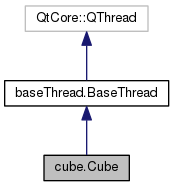
\includegraphics[width=202pt]{classcube_1_1_cube__inherit__graph}
\end{center}
\end{figure}


Collaboration diagram for cube.\-Cube\-:\nopagebreak
\begin{figure}[H]
\begin{center}
\leavevmode
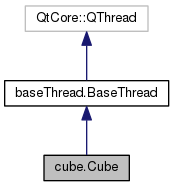
\includegraphics[width=202pt]{classcube_1_1_cube__coll__graph}
\end{center}
\end{figure}
\subsubsection*{Public Member Functions}
\begin{DoxyCompactItemize}
\item 
def \hyperlink{classcube_1_1_cube_a54d6a19cec851423c02c53f071364184}{\-\_\-\-\_\-init\-\_\-\-\_\-}
\begin{DoxyCompactList}\small\item\em Constructor. \end{DoxyCompactList}\item 
def \hyperlink{classcube_1_1_cube_a7a26b85d9e5c8699bc5e7f58bb92cdb4}{update\-Data}
\begin{DoxyCompactList}\small\item\em Gets data from serial thread. \end{DoxyCompactList}\item 
def \hyperlink{classcube_1_1_cube_a04f16dee59b9ff3ec84a913b96c997e7}{run}
\begin{DoxyCompactList}\small\item\em Main function. \end{DoxyCompactList}\item 
def \hyperlink{classcube_1_1_cube_a06759c5e77eb0aeb358521b686752004}{Init\-G\-L}
\begin{DoxyCompactList}\small\item\em Inits Open\-G\-L. \end{DoxyCompactList}\item 
def \hyperlink{classcube_1_1_cube_a08b569f052645a49639006bf11d78e6a}{display}
\begin{DoxyCompactList}\small\item\em Draws the arms with the rotation data. \end{DoxyCompactList}\item 
\hypertarget{classcube_1_1_cube_a1190ce772ca38f38358b1bad517d29e9}{def {\bfseries new\-Position}}\label{classcube_1_1_cube_a1190ce772ca38f38358b1bad517d29e9}

\item 
def \hyperlink{classcube_1_1_cube_a36bfb8dce020ea21994e63caa0275c5c}{reshape}
\item 
def \hyperlink{classcube_1_1_cube_a36d94c0f58a304cf44f34302ce824255}{Key\-Pressed}
\begin{DoxyCompactList}\small\item\em Callback for keypress events. \end{DoxyCompactList}\item 
def \hyperlink{classcube_1_1_cube_a5a9cd50b0941651a604d9671171f9810}{draw\-Forearm}
\begin{DoxyCompactList}\small\item\em Draws cube for the foreaarm representation. \end{DoxyCompactList}\item 
def \hyperlink{classcube_1_1_cube_a8bda6fd8855391222e9a1e94bac0e53f}{draw\-Arm}
\begin{DoxyCompactList}\small\item\em Draws cube for the arm representation. \end{DoxyCompactList}\item 
def \hyperlink{classcube_1_1_cube_ae58c09258290fa5e3c20c8409cf89136}{Load\-Textures}
\begin{DoxyCompactList}\small\item\em Add textures for the cube. \end{DoxyCompactList}\end{DoxyCompactItemize}
\subsubsection*{Public Attributes}
\begin{DoxyCompactItemize}
\item 
\hypertarget{classcube_1_1_cube_a0d1e3677b4638403654fc50430cae458}{{\bfseries data}}\label{classcube_1_1_cube_a0d1e3677b4638403654fc50430cae458}

\item 
\hypertarget{classcube_1_1_cube_aeffa8b0c4e591d1ff426f6554fec3431}{{\bfseries R2}}\label{classcube_1_1_cube_aeffa8b0c4e591d1ff426f6554fec3431}

\item 
\hypertarget{classcube_1_1_cube_ad952bef431eb000da224211df9e6dd78}{{\bfseries window}}\label{classcube_1_1_cube_ad952bef431eb000da224211df9e6dd78}

\end{DoxyCompactItemize}
\subsubsection*{Static Public Attributes}
\begin{DoxyCompactItemize}
\item 
\hypertarget{classcube_1_1_cube_ae25d867e3a91fa45c7c47638d5d77424}{int {\bfseries window} = 0}\label{classcube_1_1_cube_ae25d867e3a91fa45c7c47638d5d77424}

\item 
\hypertarget{classcube_1_1_cube_a9cd7bc2a19476c6b1467427579a7160e}{int {\bfseries Y} = 0}\label{classcube_1_1_cube_a9cd7bc2a19476c6b1467427579a7160e}

\item 
\hypertarget{classcube_1_1_cube_a4f694041d4ad22bcb3ae78538a3eb3da}{int {\bfseries P} = 0}\label{classcube_1_1_cube_a4f694041d4ad22bcb3ae78538a3eb3da}

\item 
\hypertarget{classcube_1_1_cube_ae784e9234aa81372e59677259716e117}{int {\bfseries R} = 0}\label{classcube_1_1_cube_ae784e9234aa81372e59677259716e117}

\item 
\hypertarget{classcube_1_1_cube_a7205513bbd828e59fd5ad263e85d8d15}{list {\bfseries L\-A\-X} = \mbox{[}0.\-0\mbox{]}}\label{classcube_1_1_cube_a7205513bbd828e59fd5ad263e85d8d15}

\item 
\hypertarget{classcube_1_1_cube_a236318ddb5e570e19f5c39ddeb226663}{list {\bfseries L\-A\-Y} = \mbox{[}0.\-0\mbox{]}}\label{classcube_1_1_cube_a236318ddb5e570e19f5c39ddeb226663}

\item 
\hypertarget{classcube_1_1_cube_a14d45fb77d96f4eac29db85bde85527f}{list {\bfseries L\-A\-Z} = \mbox{[}0.\-0\mbox{]}}\label{classcube_1_1_cube_a14d45fb77d96f4eac29db85bde85527f}

\item 
\hypertarget{classcube_1_1_cube_afdd85de2ddeec7817ce5f7af80d27b5f}{int {\bfseries X} = 0}\label{classcube_1_1_cube_afdd85de2ddeec7817ce5f7af80d27b5f}

\item 
\hypertarget{classcube_1_1_cube_a4e58c52c5e966f30927a83697e0853d5}{int {\bfseries Z} = 0}\label{classcube_1_1_cube_a4e58c52c5e966f30927a83697e0853d5}

\end{DoxyCompactItemize}


\subsubsection{Detailed Description}
Displays the orientation as a 3\-D cube. 

\subsubsection{Constructor \& Destructor Documentation}
\hypertarget{classcube_1_1_cube_a54d6a19cec851423c02c53f071364184}{\index{cube\-::\-Cube@{cube\-::\-Cube}!\-\_\-\-\_\-init\-\_\-\-\_\-@{\-\_\-\-\_\-init\-\_\-\-\_\-}}
\index{\-\_\-\-\_\-init\-\_\-\-\_\-@{\-\_\-\-\_\-init\-\_\-\-\_\-}!cube::Cube@{cube\-::\-Cube}}
\paragraph[{\-\_\-\-\_\-init\-\_\-\-\_\-}]{\setlength{\rightskip}{0pt plus 5cm}def cube.\-Cube.\-\_\-\-\_\-init\-\_\-\-\_\- (
\begin{DoxyParamCaption}
\item[{}]{self, }
\item[{}]{data}
\end{DoxyParamCaption}
)}}\label{classcube_1_1_cube_a54d6a19cec851423c02c53f071364184}


Constructor. 


\begin{DoxyParams}{Parameters}
{\em data} & Pass Serial\-Thread object to connect signal \\
\hline
\end{DoxyParams}


\subsubsection{Member Function Documentation}
\hypertarget{classcube_1_1_cube_a08b569f052645a49639006bf11d78e6a}{\index{cube\-::\-Cube@{cube\-::\-Cube}!display@{display}}
\index{display@{display}!cube::Cube@{cube\-::\-Cube}}
\paragraph[{display}]{\setlength{\rightskip}{0pt plus 5cm}def cube.\-Cube.\-display (
\begin{DoxyParamCaption}
\item[{}]{self}
\end{DoxyParamCaption}
)}}\label{classcube_1_1_cube_a08b569f052645a49639006bf11d78e6a}


Draws the arms with the rotation data. 


\begin{DoxyParams}{Parameters}
{\em self} & The object pointer. \\
\hline
\end{DoxyParams}
\hypertarget{classcube_1_1_cube_a8bda6fd8855391222e9a1e94bac0e53f}{\index{cube\-::\-Cube@{cube\-::\-Cube}!draw\-Arm@{draw\-Arm}}
\index{draw\-Arm@{draw\-Arm}!cube::Cube@{cube\-::\-Cube}}
\paragraph[{draw\-Arm}]{\setlength{\rightskip}{0pt plus 5cm}def cube.\-Cube.\-draw\-Arm (
\begin{DoxyParamCaption}
\item[{}]{self}
\end{DoxyParamCaption}
)}}\label{classcube_1_1_cube_a8bda6fd8855391222e9a1e94bac0e53f}


Draws cube for the arm representation. 


\begin{DoxyParams}{Parameters}
{\em self} & The object pointer. \\
\hline
\end{DoxyParams}
\hypertarget{classcube_1_1_cube_a5a9cd50b0941651a604d9671171f9810}{\index{cube\-::\-Cube@{cube\-::\-Cube}!draw\-Forearm@{draw\-Forearm}}
\index{draw\-Forearm@{draw\-Forearm}!cube::Cube@{cube\-::\-Cube}}
\paragraph[{draw\-Forearm}]{\setlength{\rightskip}{0pt plus 5cm}def cube.\-Cube.\-draw\-Forearm (
\begin{DoxyParamCaption}
\item[{}]{self}
\end{DoxyParamCaption}
)}}\label{classcube_1_1_cube_a5a9cd50b0941651a604d9671171f9810}


Draws cube for the foreaarm representation. 


\begin{DoxyParams}{Parameters}
{\em self} & The object pointer. \\
\hline
\end{DoxyParams}
\hypertarget{classcube_1_1_cube_a06759c5e77eb0aeb358521b686752004}{\index{cube\-::\-Cube@{cube\-::\-Cube}!Init\-G\-L@{Init\-G\-L}}
\index{Init\-G\-L@{Init\-G\-L}!cube::Cube@{cube\-::\-Cube}}
\paragraph[{Init\-G\-L}]{\setlength{\rightskip}{0pt plus 5cm}def cube.\-Cube.\-Init\-G\-L (
\begin{DoxyParamCaption}
\item[{}]{self, }
\item[{}]{Width, }
\item[{}]{Height}
\end{DoxyParamCaption}
)}}\label{classcube_1_1_cube_a06759c5e77eb0aeb358521b686752004}


Inits Open\-G\-L. 


\begin{DoxyParams}{Parameters}
{\em self} & The object pointer. \\
\hline
{\em Width} & size of the Window \\
\hline
{\em Height} & size of the Window \\
\hline
\end{DoxyParams}
\hypertarget{classcube_1_1_cube_a36d94c0f58a304cf44f34302ce824255}{\index{cube\-::\-Cube@{cube\-::\-Cube}!Key\-Pressed@{Key\-Pressed}}
\index{Key\-Pressed@{Key\-Pressed}!cube::Cube@{cube\-::\-Cube}}
\paragraph[{Key\-Pressed}]{\setlength{\rightskip}{0pt plus 5cm}def cube.\-Cube.\-Key\-Pressed (
\begin{DoxyParamCaption}
\item[{}]{self, }
\item[{}]{args}
\end{DoxyParamCaption}
)}}\label{classcube_1_1_cube_a36d94c0f58a304cf44f34302ce824255}


Callback for keypress events. 


\begin{DoxyParams}{Parameters}
{\em self} & The object pointer. \\
\hline
{\em args} & Pointer to the args for accesing input data \\
\hline
\end{DoxyParams}
\hypertarget{classcube_1_1_cube_ae58c09258290fa5e3c20c8409cf89136}{\index{cube\-::\-Cube@{cube\-::\-Cube}!Load\-Textures@{Load\-Textures}}
\index{Load\-Textures@{Load\-Textures}!cube::Cube@{cube\-::\-Cube}}
\paragraph[{Load\-Textures}]{\setlength{\rightskip}{0pt plus 5cm}def cube.\-Cube.\-Load\-Textures (
\begin{DoxyParamCaption}
\item[{}]{self}
\end{DoxyParamCaption}
)}}\label{classcube_1_1_cube_ae58c09258290fa5e3c20c8409cf89136}


Add textures for the cube. 

Applies a png image as a texture for the faces of the cube \begin{DoxyNote}{Note}
experimental 
\end{DoxyNote}

\begin{DoxyParams}{Parameters}
{\em self} & The object pointer. \\
\hline
\end{DoxyParams}
\hypertarget{classcube_1_1_cube_a36bfb8dce020ea21994e63caa0275c5c}{\index{cube\-::\-Cube@{cube\-::\-Cube}!reshape@{reshape}}
\index{reshape@{reshape}!cube::Cube@{cube\-::\-Cube}}
\paragraph[{reshape}]{\setlength{\rightskip}{0pt plus 5cm}def cube.\-Cube.\-reshape (
\begin{DoxyParamCaption}
\item[{}]{self, }
\item[{}]{Width, }
\item[{}]{Height}
\end{DoxyParamCaption}
)}}\label{classcube_1_1_cube_a36bfb8dce020ea21994e63caa0275c5c}

\begin{DoxyParams}{Parameters}
{\em self} & The object pointer. \\
\hline
{\em Width} & size of the Window \\
\hline
{\em Height} & size of the Window \\
\hline
\end{DoxyParams}
\hypertarget{classcube_1_1_cube_a04f16dee59b9ff3ec84a913b96c997e7}{\index{cube\-::\-Cube@{cube\-::\-Cube}!run@{run}}
\index{run@{run}!cube::Cube@{cube\-::\-Cube}}
\paragraph[{run}]{\setlength{\rightskip}{0pt plus 5cm}def cube.\-Cube.\-run (
\begin{DoxyParamCaption}
\item[{}]{self}
\end{DoxyParamCaption}
)}}\label{classcube_1_1_cube_a04f16dee59b9ff3ec84a913b96c997e7}


Main function. 

Inits and configures all the G\-L\-U\-T parameters to and defines the associated functions to each event 
\begin{DoxyParams}{Parameters}
{\em self} & The object pointer. \\
\hline
\end{DoxyParams}
\hypertarget{classcube_1_1_cube_a7a26b85d9e5c8699bc5e7f58bb92cdb4}{\index{cube\-::\-Cube@{cube\-::\-Cube}!update\-Data@{update\-Data}}
\index{update\-Data@{update\-Data}!cube::Cube@{cube\-::\-Cube}}
\paragraph[{update\-Data}]{\setlength{\rightskip}{0pt plus 5cm}def cube.\-Cube.\-update\-Data (
\begin{DoxyParamCaption}
\item[{}]{self}
\end{DoxyParamCaption}
)}}\label{classcube_1_1_cube_a7a26b85d9e5c8699bc5e7f58bb92cdb4}


Gets data from serial thread. 


\begin{DoxyParams}{Parameters}
{\em self} & The object pointer. \\
\hline
\end{DoxyParams}


The documentation for this class was generated from the following file\-:\begin{DoxyCompactItemize}
\item 
I\-M\-U\-Graph/cube.\-py\end{DoxyCompactItemize}

\hypertarget{classfall_detection_1_1_fall_detection}{\subsection{fall\-Detection.\-Fall\-Detection Class Reference}
\label{classfall_detection_1_1_fall_detection}\index{fall\-Detection.\-Fall\-Detection@{fall\-Detection.\-Fall\-Detection}}
}


Detects fall from the accelerometer data.  


\subsubsection*{Public Member Functions}
\begin{DoxyCompactItemize}
\item 
def \hyperlink{classfall_detection_1_1_fall_detection_a3bdf921ddeab54c9eb78231e64e3f8c1}{\-\_\-\-\_\-init\-\_\-\-\_\-}
\begin{DoxyCompactList}\small\item\em Constructor for the Fall Detection algorithm. \end{DoxyCompactList}\item 
def \hyperlink{classfall_detection_1_1_fall_detection_a47ae3cde72ec28563e117e16d9e0d962}{normal\-Vector}
\begin{DoxyCompactList}\small\item\em Calculates de normal vector of three vectors. \end{DoxyCompactList}\item 
def \hyperlink{classfall_detection_1_1_fall_detection_aad3c9071e7a676843cdd968fef66bb56}{search1\-L\-F\-T}
\begin{DoxyCompactList}\small\item\em Finds the first lower value on a list. \end{DoxyCompactList}\item 
def \hyperlink{classfall_detection_1_1_fall_detection_a15d331e7cde45376a1ed81628f4fd37b}{search2\-L\-F\-T}
\begin{DoxyCompactList}\small\item\em Finds the first upper value on a list. \end{DoxyCompactList}\item 
def \hyperlink{classfall_detection_1_1_fall_detection_ace430c2a9f1d9d20e5ef1794693a0895}{update\-Fall}
\begin{DoxyCompactList}\small\item\em Updates the Fall Detection algorithm with the last data. \end{DoxyCompactList}\item 
def \hyperlink{classfall_detection_1_1_fall_detection_a0563f1d15637964895896b45581bd267}{get\-Fall\-Status}
\begin{DoxyCompactList}\small\item\em Getter for the fall status obtained from the last update. \end{DoxyCompactList}\item 
def \hyperlink{classfall_detection_1_1_fall_detection_aa9bad5034e22fa59b7f54f66c9d3c042}{get\-Semi\-Fall\-Status}
\begin{DoxyCompactList}\small\item\em Getter for the semi fall status obtained from the last update. \end{DoxyCompactList}\end{DoxyCompactItemize}
\subsubsection*{Public Attributes}
\begin{DoxyCompactItemize}
\item 
\hypertarget{classfall_detection_1_1_fall_detection_a957affda8f3d78b80055b7ca0b3b3e48}{{\bfseries U\-F\-T}}\label{classfall_detection_1_1_fall_detection_a957affda8f3d78b80055b7ca0b3b3e48}

\item 
\hypertarget{classfall_detection_1_1_fall_detection_a7a7839c4cad6c984c0b4086f1633bc13}{{\bfseries L\-F\-T}}\label{classfall_detection_1_1_fall_detection_a7a7839c4cad6c984c0b4086f1633bc13}

\item 
\hypertarget{classfall_detection_1_1_fall_detection_a8211460c1e22f409e204e4dd9e5843c0}{{\bfseries fs}}\label{classfall_detection_1_1_fall_detection_a8211460c1e22f409e204e4dd9e5843c0}

\item 
\hypertarget{classfall_detection_1_1_fall_detection_a9c34ba457d991bc7d1bdafe95eb1d2d8}{{\bfseries P\-O\-S\-I\-T\-I\-O\-N}}\label{classfall_detection_1_1_fall_detection_a9c34ba457d991bc7d1bdafe95eb1d2d8}

\end{DoxyCompactItemize}
\subsubsection*{Static Public Attributes}
\begin{DoxyCompactItemize}
\item 
int \hyperlink{classfall_detection_1_1_fall_detection_aa99e61fc17e5b0a0e42c148be47ffdd5}{S\-I\-Z\-E} = 1024
\begin{DoxyCompactList}\small\item\em Buffer size for S\-V. \end{DoxyCompactList}\item 
float \hyperlink{classfall_detection_1_1_fall_detection_a34f4c16af8de8c4efaf6779c46ef5f48}{U\-F\-T} = 2.\-8
\begin{DoxyCompactList}\small\item\em Upper force trigger. \end{DoxyCompactList}\item 
float \hyperlink{classfall_detection_1_1_fall_detection_a32fb8ad5bc5820480e2eb450c679eeda}{L\-F\-T} = 0.\-65
\begin{DoxyCompactList}\small\item\em Lower force trigger. \end{DoxyCompactList}\item 
int \hyperlink{classfall_detection_1_1_fall_detection_aedf3abe0136fa5efe23df8f35228d4a6}{fs} = .\-02
\begin{DoxyCompactList}\small\item\em Time between samples. \end{DoxyCompactList}\item 
list \hyperlink{classfall_detection_1_1_fall_detection_a343631714c9cc3129eaa46abe5c5db82}{S\-V} = \mbox{[}0.\-0\mbox{]}
\begin{DoxyCompactList}\small\item\em List for S\-V values. \end{DoxyCompactList}\item 
\hypertarget{classfall_detection_1_1_fall_detection_addb95520ce608393fd378aed70293199}{list \hyperlink{classfall_detection_1_1_fall_detection_addb95520ce608393fd378aed70293199}{Y\-A\-W} = \mbox{[}.\-0\mbox{]}}\label{classfall_detection_1_1_fall_detection_addb95520ce608393fd378aed70293199}

\begin{DoxyCompactList}\small\item\em List for angles monitoring posture. \end{DoxyCompactList}\item 
\hypertarget{classfall_detection_1_1_fall_detection_aa9fba49d5c83db3cc9032ede9c7d3ff8}{list {\bfseries P\-I\-T\-C\-H} = \mbox{[}.\-0\mbox{]}}\label{classfall_detection_1_1_fall_detection_aa9fba49d5c83db3cc9032ede9c7d3ff8}

\item 
\hypertarget{classfall_detection_1_1_fall_detection_aa44f488c9296cf9c27f037ae246d1649}{list {\bfseries R\-O\-L\-L} = \mbox{[}.\-0\mbox{]}}\label{classfall_detection_1_1_fall_detection_aa44f488c9296cf9c27f037ae246d1649}

\item 
\hypertarget{classfall_detection_1_1_fall_detection_a529e246a5c2c87bdb5c6426abeeb8dfb}{int \hyperlink{classfall_detection_1_1_fall_detection_a529e246a5c2c87bdb5c6426abeeb8dfb}{P\-O\-S\-I\-T\-I\-O\-N} = 0}\label{classfall_detection_1_1_fall_detection_a529e246a5c2c87bdb5c6426abeeb8dfb}

\begin{DoxyCompactList}\small\item\em Indicates for the buffers index. \end{DoxyCompactList}\item 
\hyperlink{classfall_detection_1_1_fall_detection_afa9560adcae4144df3ba9a753c920060}{D\-R\-O\-P} = False
\begin{DoxyCompactList}\small\item\em Indicates if a fall was detected. \end{DoxyCompactList}\item 
\hypertarget{classfall_detection_1_1_fall_detection_a2d6eb7f362620d5992fc5d6ab4d5880b}{{\bfseries S\-E\-M\-I\-D\-R\-O\-P} = False}\label{classfall_detection_1_1_fall_detection_a2d6eb7f362620d5992fc5d6ab4d5880b}

\end{DoxyCompactItemize}


\subsubsection{Detailed Description}
Detects fall from the accelerometer data. 

Using an accelerometer calculates\-:
\begin{DoxyItemize}
\item Impact normalized force (S\-V) and impact ranges (U\-F\-T, L\-F\-T)
\item Detectes a range of time during the detected impact (tm, ti)
\item Determinates the speed of the fall during the fallind time (V0)
\item Detect the posture (change in orientation) respect the initial impact posture. With all these data and determinations is possible to estimate with presition a fall and impact.
\end{DoxyItemize}

\begin{DoxyAuthor}{Author}
Dr. Pablo Reyes 

Sebastian Sepulveda 
\end{DoxyAuthor}
\begin{DoxyRefDesc}{Todo}
\item[\hyperlink{todo__todo000003}{Todo}]Validate algorithms \end{DoxyRefDesc}


\subsubsection{Constructor \& Destructor Documentation}
\hypertarget{classfall_detection_1_1_fall_detection_a3bdf921ddeab54c9eb78231e64e3f8c1}{\index{fall\-Detection\-::\-Fall\-Detection@{fall\-Detection\-::\-Fall\-Detection}!\-\_\-\-\_\-init\-\_\-\-\_\-@{\-\_\-\-\_\-init\-\_\-\-\_\-}}
\index{\-\_\-\-\_\-init\-\_\-\-\_\-@{\-\_\-\-\_\-init\-\_\-\-\_\-}!fallDetection::FallDetection@{fall\-Detection\-::\-Fall\-Detection}}
\paragraph[{\-\_\-\-\_\-init\-\_\-\-\_\-}]{\setlength{\rightskip}{0pt plus 5cm}def fall\-Detection.\-Fall\-Detection.\-\_\-\-\_\-init\-\_\-\-\_\- (
\begin{DoxyParamCaption}
\item[{}]{self, }
\item[{}]{fs = {\ttfamily .02}, }
\item[{}]{U\-F\-T = {\ttfamily 2.8}, }
\item[{}]{L\-F\-T = {\ttfamily .65}}
\end{DoxyParamCaption}
)}}\label{classfall_detection_1_1_fall_detection_a3bdf921ddeab54c9eb78231e64e3f8c1}


Constructor for the Fall Detection algorithm. 

Initializes the values of fs, U\-F\-T and L\-F\-T allowing to change the default values of the algorithms 
\begin{DoxyParams}{Parameters}
{\em self} & The object pointer \\
\hline
{\em fs} & Time between samples, in seconds \\
\hline
{\em U\-F\-T} & U\-F\-T trigger, in g (gravities) \\
\hline
{\em L\-F\-T} & L\-F\-T trigger, in g (gravities) \\
\hline
\end{DoxyParams}


\subsubsection{Member Function Documentation}
\hypertarget{classfall_detection_1_1_fall_detection_a0563f1d15637964895896b45581bd267}{\index{fall\-Detection\-::\-Fall\-Detection@{fall\-Detection\-::\-Fall\-Detection}!get\-Fall\-Status@{get\-Fall\-Status}}
\index{get\-Fall\-Status@{get\-Fall\-Status}!fallDetection::FallDetection@{fall\-Detection\-::\-Fall\-Detection}}
\paragraph[{get\-Fall\-Status}]{\setlength{\rightskip}{0pt plus 5cm}def fall\-Detection.\-Fall\-Detection.\-get\-Fall\-Status (
\begin{DoxyParamCaption}
\item[{}]{self}
\end{DoxyParamCaption}
)}}\label{classfall_detection_1_1_fall_detection_a0563f1d15637964895896b45581bd267}


Getter for the fall status obtained from the last update. 

Return the result of the Fall Detection algorithm from the last \hyperlink{classfall_detection_1_1_fall_detection_ace430c2a9f1d9d20e5ef1794693a0895}{update\-Fall} call. \begin{DoxyReturn}{Returns}
Status of the fall
\begin{DoxyItemize}
\item {\bfseries T\-R\-U\-E} \-: if a fall was detected
\item {\bfseries F\-A\-L\-S\-E} \-: if a fall wasn't detected 
\end{DoxyItemize}
\end{DoxyReturn}
\hypertarget{classfall_detection_1_1_fall_detection_aa9bad5034e22fa59b7f54f66c9d3c042}{\index{fall\-Detection\-::\-Fall\-Detection@{fall\-Detection\-::\-Fall\-Detection}!get\-Semi\-Fall\-Status@{get\-Semi\-Fall\-Status}}
\index{get\-Semi\-Fall\-Status@{get\-Semi\-Fall\-Status}!fallDetection::FallDetection@{fall\-Detection\-::\-Fall\-Detection}}
\paragraph[{get\-Semi\-Fall\-Status}]{\setlength{\rightskip}{0pt plus 5cm}def fall\-Detection.\-Fall\-Detection.\-get\-Semi\-Fall\-Status (
\begin{DoxyParamCaption}
\item[{}]{self}
\end{DoxyParamCaption}
)}}\label{classfall_detection_1_1_fall_detection_aa9bad5034e22fa59b7f54f66c9d3c042}


Getter for the semi fall status obtained from the last update. 

Return the result of the Fall Detection algorithm from the last \hyperlink{classfall_detection_1_1_fall_detection_ace430c2a9f1d9d20e5ef1794693a0895}{update\-Fall} call before checking the posture \begin{DoxyReturn}{Returns}
Status of the semi fall
\begin{DoxyItemize}
\item {\bfseries T\-R\-U\-E} \-: if a semi fall was detected
\item {\bfseries F\-A\-L\-S\-E} \-: if a semi fall wasn't detected 
\end{DoxyItemize}
\end{DoxyReturn}
\hypertarget{classfall_detection_1_1_fall_detection_a47ae3cde72ec28563e117e16d9e0d962}{\index{fall\-Detection\-::\-Fall\-Detection@{fall\-Detection\-::\-Fall\-Detection}!normal\-Vector@{normal\-Vector}}
\index{normal\-Vector@{normal\-Vector}!fallDetection::FallDetection@{fall\-Detection\-::\-Fall\-Detection}}
\paragraph[{normal\-Vector}]{\setlength{\rightskip}{0pt plus 5cm}def fall\-Detection.\-Fall\-Detection.\-normal\-Vector (
\begin{DoxyParamCaption}
\item[{}]{self, }
\item[{}]{x, }
\item[{}]{y, }
\item[{}]{z}
\end{DoxyParamCaption}
)}}\label{classfall_detection_1_1_fall_detection_a47ae3cde72ec28563e117e16d9e0d962}


Calculates de normal vector of three vectors. 

Uses the math library from Python 
\begin{DoxyParams}{Parameters}
{\em self} & The objetc pointer \\
\hline
{\em x} & 1st value to normalize \\
\hline
{\em y} & 2nd value to normalize \\
\hline
{\em z} & 3rd value to normalize \\
\hline
\end{DoxyParams}
\begin{DoxyReturn}{Returns}
Normalized value of x,y and z 
\end{DoxyReturn}
\hypertarget{classfall_detection_1_1_fall_detection_aad3c9071e7a676843cdd968fef66bb56}{\index{fall\-Detection\-::\-Fall\-Detection@{fall\-Detection\-::\-Fall\-Detection}!search1\-L\-F\-T@{search1\-L\-F\-T}}
\index{search1\-L\-F\-T@{search1\-L\-F\-T}!fallDetection::FallDetection@{fall\-Detection\-::\-Fall\-Detection}}
\paragraph[{search1\-L\-F\-T}]{\setlength{\rightskip}{0pt plus 5cm}def fall\-Detection.\-Fall\-Detection.\-search1\-L\-F\-T (
\begin{DoxyParamCaption}
\item[{}]{self, }
\item[{}]{value, }
\item[{}]{vector}
\end{DoxyParamCaption}
)}}\label{classfall_detection_1_1_fall_detection_aad3c9071e7a676843cdd968fef66bb56}


Finds the first lower value on a list. 

Finds the first lower value of L\-F\-T on a list 
\begin{DoxyParams}{Parameters}
{\em self} & The objetc pointer \\
\hline
{\em value} & The value to find in the list \\
\hline
{\em vector} & The list to find on \\
\hline
\end{DoxyParams}
\begin{DoxyReturn}{Returns}
The index where the value (or 1st lower) was found 
\end{DoxyReturn}
\hypertarget{classfall_detection_1_1_fall_detection_a15d331e7cde45376a1ed81628f4fd37b}{\index{fall\-Detection\-::\-Fall\-Detection@{fall\-Detection\-::\-Fall\-Detection}!search2\-L\-F\-T@{search2\-L\-F\-T}}
\index{search2\-L\-F\-T@{search2\-L\-F\-T}!fallDetection::FallDetection@{fall\-Detection\-::\-Fall\-Detection}}
\paragraph[{search2\-L\-F\-T}]{\setlength{\rightskip}{0pt plus 5cm}def fall\-Detection.\-Fall\-Detection.\-search2\-L\-F\-T (
\begin{DoxyParamCaption}
\item[{}]{self, }
\item[{}]{value, }
\item[{}]{vector}
\end{DoxyParamCaption}
)}}\label{classfall_detection_1_1_fall_detection_a15d331e7cde45376a1ed81628f4fd37b}


Finds the first upper value on a list. 

Finds the first upper value of L\-F\-T on a list 
\begin{DoxyParams}{Parameters}
{\em self} & The objetc pointer \\
\hline
{\em value} & The value to find in the list \\
\hline
{\em vector} & The list to find on \\
\hline
\end{DoxyParams}
\begin{DoxyReturn}{Returns}
The index where the value (or 1st upper) was found 
\end{DoxyReturn}
\hypertarget{classfall_detection_1_1_fall_detection_ace430c2a9f1d9d20e5ef1794693a0895}{\index{fall\-Detection\-::\-Fall\-Detection@{fall\-Detection\-::\-Fall\-Detection}!update\-Fall@{update\-Fall}}
\index{update\-Fall@{update\-Fall}!fallDetection::FallDetection@{fall\-Detection\-::\-Fall\-Detection}}
\paragraph[{update\-Fall}]{\setlength{\rightskip}{0pt plus 5cm}def fall\-Detection.\-Fall\-Detection.\-update\-Fall (
\begin{DoxyParamCaption}
\item[{}]{self, }
\item[{}]{x, }
\item[{}]{y, }
\item[{}]{z, }
\item[{}]{yaw, }
\item[{}]{pitch, }
\item[{}]{roll}
\end{DoxyParamCaption}
)}}\label{classfall_detection_1_1_fall_detection_ace430c2a9f1d9d20e5ef1794693a0895}


Updates the Fall Detection algorithm with the last data. 

The function searches for a S\-V in between the impact range, a fall speed between the time corresponding the impact and the posture when a fall is detected.


\begin{DoxyParams}{Parameters}
{\em self} & The objetc pointer \\
\hline
{\em x} & acceleration in X axis, in g (gravities) \\
\hline
{\em y} & acceleration in Y axis, in g (gravities) \\
\hline
{\em z} & acceleration in Z axis, in g (gravities)\\
\hline
\end{DoxyParams}
\begin{DoxyNote}{Note}
The algorithm proposed sugest to filter the adquired data with a lowpass 1st order butterworth at 100 Hz. The data adquired from the M\-P\-U-\/9150 (or even A\-D\-X\-L-\/345) digital accelerometers can (and is) configured to filter the data and outputs filtered raw data. Therefore, this filter is not implemented. 

The algorithm has been implemented asumming a sensor fusion running continusly for obtaining yaw, pitch, roll. The class stores the data in a buffer for look back at the posture. 
\end{DoxyNote}


\subsubsection{Member Data Documentation}
\hypertarget{classfall_detection_1_1_fall_detection_afa9560adcae4144df3ba9a753c920060}{\index{fall\-Detection\-::\-Fall\-Detection@{fall\-Detection\-::\-Fall\-Detection}!D\-R\-O\-P@{D\-R\-O\-P}}
\index{D\-R\-O\-P@{D\-R\-O\-P}!fallDetection::FallDetection@{fall\-Detection\-::\-Fall\-Detection}}
\paragraph[{D\-R\-O\-P}]{\setlength{\rightskip}{0pt plus 5cm}fall\-Detection.\-Fall\-Detection.\-D\-R\-O\-P = False\hspace{0.3cm}{\ttfamily [static]}}}\label{classfall_detection_1_1_fall_detection_afa9560adcae4144df3ba9a753c920060}


Indicates if a fall was detected. 


\begin{DoxyItemize}
\item if {\bfseries T\-R\-U\-E\-:} a fall was detected
\item if {\bfseries F\-A\-L\-L\-:} a fall wasn't detected 
\end{DoxyItemize}\hypertarget{classfall_detection_1_1_fall_detection_aedf3abe0136fa5efe23df8f35228d4a6}{\index{fall\-Detection\-::\-Fall\-Detection@{fall\-Detection\-::\-Fall\-Detection}!fs@{fs}}
\index{fs@{fs}!fallDetection::FallDetection@{fall\-Detection\-::\-Fall\-Detection}}
\paragraph[{fs}]{\setlength{\rightskip}{0pt plus 5cm}int fall\-Detection.\-Fall\-Detection.\-fs = .\-02\hspace{0.3cm}{\ttfamily [static]}}}\label{classfall_detection_1_1_fall_detection_aedf3abe0136fa5efe23df8f35228d4a6}


Time between samples. 

Time between samples, in seconds \hypertarget{classfall_detection_1_1_fall_detection_a32fb8ad5bc5820480e2eb450c679eeda}{\index{fall\-Detection\-::\-Fall\-Detection@{fall\-Detection\-::\-Fall\-Detection}!L\-F\-T@{L\-F\-T}}
\index{L\-F\-T@{L\-F\-T}!fallDetection::FallDetection@{fall\-Detection\-::\-Fall\-Detection}}
\paragraph[{L\-F\-T}]{\setlength{\rightskip}{0pt plus 5cm}float fall\-Detection.\-Fall\-Detection.\-L\-F\-T = 0.\-65\hspace{0.3cm}{\ttfamily [static]}}}\label{classfall_detection_1_1_fall_detection_a32fb8ad5bc5820480e2eb450c679eeda}


Lower force trigger. 

Lower force trigger for detecting the start of the impact, in g (gravities) \hypertarget{classfall_detection_1_1_fall_detection_aa99e61fc17e5b0a0e42c148be47ffdd5}{\index{fall\-Detection\-::\-Fall\-Detection@{fall\-Detection\-::\-Fall\-Detection}!S\-I\-Z\-E@{S\-I\-Z\-E}}
\index{S\-I\-Z\-E@{S\-I\-Z\-E}!fallDetection::FallDetection@{fall\-Detection\-::\-Fall\-Detection}}
\paragraph[{S\-I\-Z\-E}]{\setlength{\rightskip}{0pt plus 5cm}int fall\-Detection.\-Fall\-Detection.\-S\-I\-Z\-E = 1024\hspace{0.3cm}{\ttfamily [static]}}}\label{classfall_detection_1_1_fall_detection_aa99e61fc17e5b0a0e42c148be47ffdd5}


Buffer size for S\-V. 

Determinate the buffer size for storing the S\-V data \hypertarget{classfall_detection_1_1_fall_detection_a343631714c9cc3129eaa46abe5c5db82}{\index{fall\-Detection\-::\-Fall\-Detection@{fall\-Detection\-::\-Fall\-Detection}!S\-V@{S\-V}}
\index{S\-V@{S\-V}!fallDetection::FallDetection@{fall\-Detection\-::\-Fall\-Detection}}
\paragraph[{S\-V}]{\setlength{\rightskip}{0pt plus 5cm}list fall\-Detection.\-Fall\-Detection.\-S\-V = \mbox{[}0.\-0\mbox{]}\hspace{0.3cm}{\ttfamily [static]}}}\label{classfall_detection_1_1_fall_detection_a343631714c9cc3129eaa46abe5c5db82}


List for S\-V values. 

Stores the last S\-V values \hypertarget{classfall_detection_1_1_fall_detection_a34f4c16af8de8c4efaf6779c46ef5f48}{\index{fall\-Detection\-::\-Fall\-Detection@{fall\-Detection\-::\-Fall\-Detection}!U\-F\-T@{U\-F\-T}}
\index{U\-F\-T@{U\-F\-T}!fallDetection::FallDetection@{fall\-Detection\-::\-Fall\-Detection}}
\paragraph[{U\-F\-T}]{\setlength{\rightskip}{0pt plus 5cm}float fall\-Detection.\-Fall\-Detection.\-U\-F\-T = 2.\-8\hspace{0.3cm}{\ttfamily [static]}}}\label{classfall_detection_1_1_fall_detection_a34f4c16af8de8c4efaf6779c46ef5f48}


Upper force trigger. 

Upper force trigger for detecting an impact, in g (gravities) 

The documentation for this class was generated from the following file\-:\begin{DoxyCompactItemize}
\item 
I\-M\-U\-Graph/fall\-Detection.\-py\end{DoxyCompactItemize}

\hypertarget{classimu_1_1_i_m_u}{\subsection{imu.\-I\-M\-U Class Reference}
\label{classimu_1_1_i_m_u}\index{imu.\-I\-M\-U@{imu.\-I\-M\-U}}
}


\hyperlink{classimu_1_1_i_m_u}{I\-M\-U} values for scales and data structure in the C\-S\-V data received.  


\subsubsection*{Public Member Functions}
\begin{DoxyCompactItemize}
\item 
def \hyperlink{classimu_1_1_i_m_u_a59e33a38d9043a4db299417f0042cf89}{\-\_\-\-\_\-init\-\_\-\-\_\-}
\begin{DoxyCompactList}\small\item\em Constructor. \end{DoxyCompactList}\item 
\hypertarget{classimu_1_1_i_m_u_aab7bfabaa5beb47d4868f72a431e31aa}{def {\bfseries get\-Scale\-Vector}}\label{classimu_1_1_i_m_u_aab7bfabaa5beb47d4868f72a431e31aa}

\item 
\hypertarget{classimu_1_1_i_m_u_ad9dae316b5fe3e6fd1c5370c86426b9c}{def {\bfseries get\-Range\-Accelerometer}}\label{classimu_1_1_i_m_u_ad9dae316b5fe3e6fd1c5370c86426b9c}

\item 
\hypertarget{classimu_1_1_i_m_u_a67e0f3567b12280d300f2d2f68a0ce99}{def {\bfseries get\-Range\-Gyroscope}}\label{classimu_1_1_i_m_u_a67e0f3567b12280d300f2d2f68a0ce99}

\item 
\hypertarget{classimu_1_1_i_m_u_ac5c8b889f5a3c4a0210b3b6f83f963e9}{def {\bfseries get\-Range\-Magnetometer}}\label{classimu_1_1_i_m_u_ac5c8b889f5a3c4a0210b3b6f83f963e9}

\item 
\hypertarget{classimu_1_1_i_m_u_adab7ee8a62d6636ff4d112df2ebe1b1b}{def {\bfseries get\-Range\-Euler}}\label{classimu_1_1_i_m_u_adab7ee8a62d6636ff4d112df2ebe1b1b}

\end{DoxyCompactItemize}
\subsubsection*{Public Attributes}
\begin{DoxyCompactItemize}
\item 
\hypertarget{classimu_1_1_i_m_u_a56ee9334633645e75cc52b77dab6a0a9}{{\bfseries name}}\label{classimu_1_1_i_m_u_a56ee9334633645e75cc52b77dab6a0a9}

\item 
\hypertarget{classimu_1_1_i_m_u_a78fe9612fe77fbb3513e50b21103b0df}{{\bfseries A\-C\-C\-E\-L}}\label{classimu_1_1_i_m_u_a78fe9612fe77fbb3513e50b21103b0df}

\item 
\hypertarget{classimu_1_1_i_m_u_a44efe2cd66bf3199e31f1e4b82600315}{{\bfseries G\-Y\-R\-O}}\label{classimu_1_1_i_m_u_a44efe2cd66bf3199e31f1e4b82600315}

\item 
\hypertarget{classimu_1_1_i_m_u_ac0efbd1a44c2efc5d75c130075b2323b}{{\bfseries M\-A\-G\-\_\-\-T}}\label{classimu_1_1_i_m_u_ac0efbd1a44c2efc5d75c130075b2323b}

\item 
\hypertarget{classimu_1_1_i_m_u_a5153e7b6984edaec90c75dc045d67aa0}{{\bfseries M\-A\-G\-\_\-\-G\-S}}\label{classimu_1_1_i_m_u_a5153e7b6984edaec90c75dc045d67aa0}

\item 
\hypertarget{classimu_1_1_i_m_u_a3ad9596d6d7503e43c65191eecd62bad}{{\bfseries E\-U\-L\-E\-R}}\label{classimu_1_1_i_m_u_a3ad9596d6d7503e43c65191eecd62bad}

\item 
\hypertarget{classimu_1_1_i_m_u_ac23a6625ee15c27650697e6a3f03c05c}{{\bfseries S\-C\-A\-L\-E\-\_\-\-V\-E\-C\-T\-O\-R}}\label{classimu_1_1_i_m_u_ac23a6625ee15c27650697e6a3f03c05c}

\item 
\hypertarget{classimu_1_1_i_m_u_a3b57a83b9032094704c1ffb69bfdc2ff}{{\bfseries A\-C\-C\-E\-L\-\_\-\-R\-A\-N\-G\-E}}\label{classimu_1_1_i_m_u_a3b57a83b9032094704c1ffb69bfdc2ff}

\item 
\hypertarget{classimu_1_1_i_m_u_af48a31ed24757c5fdd6471cf1904f55b}{{\bfseries G\-Y\-R\-O\-\_\-\-R\-A\-N\-G\-E}}\label{classimu_1_1_i_m_u_af48a31ed24757c5fdd6471cf1904f55b}

\item 
\hypertarget{classimu_1_1_i_m_u_ab2d0d36c888385ce9c3f40cd5050b24a}{{\bfseries M\-A\-G\-\_\-\-R\-A\-N\-G\-E}}\label{classimu_1_1_i_m_u_ab2d0d36c888385ce9c3f40cd5050b24a}

\item 
\hypertarget{classimu_1_1_i_m_u_ac4fc42bf95839b423f101a7b09e67854}{{\bfseries E\-U\-L\-E\-R\-\_\-\-R\-A\-N\-G\-E}}\label{classimu_1_1_i_m_u_ac4fc42bf95839b423f101a7b09e67854}

\end{DoxyCompactItemize}


\subsubsection{Detailed Description}
\hyperlink{classimu_1_1_i_m_u}{I\-M\-U} values for scales and data structure in the C\-S\-V data received. 

Receives a \hyperlink{classimu_1_1_i_m_u}{I\-M\-U} device name and returns data for scaling each type of data and the correct placement in the C\-S\-V format.

Also fixes inverted and swaped axis. 

\subsubsection{Constructor \& Destructor Documentation}
\hypertarget{classimu_1_1_i_m_u_a59e33a38d9043a4db299417f0042cf89}{\index{imu\-::\-I\-M\-U@{imu\-::\-I\-M\-U}!\-\_\-\-\_\-init\-\_\-\-\_\-@{\-\_\-\-\_\-init\-\_\-\-\_\-}}
\index{\-\_\-\-\_\-init\-\_\-\-\_\-@{\-\_\-\-\_\-init\-\_\-\-\_\-}!imu::IMU@{imu\-::\-I\-M\-U}}
\paragraph[{\-\_\-\-\_\-init\-\_\-\-\_\-}]{\setlength{\rightskip}{0pt plus 5cm}def imu.\-I\-M\-U.\-\_\-\-\_\-init\-\_\-\-\_\- (
\begin{DoxyParamCaption}
\item[{}]{self, }
\item[{}]{name = {\ttfamily 'MPU-\/9150'}}
\end{DoxyParamCaption}
)}}\label{classimu_1_1_i_m_u_a59e33a38d9043a4db299417f0042cf89}


Constructor. 

Creates a self.\-S\-C\-A\-L\-E\-\_\-\-V\-E\-C\-T\-O\-R for scaling the data based on the \hyperlink{classimu_1_1_i_m_u}{I\-M\-U} devices and the arregement on the C\-S\-V format. 
\begin{DoxyParams}{Parameters}
{\em self} & The object pointer \\
\hline
{\em name} & \hyperlink{classimu_1_1_i_m_u}{I\-M\-U} decive used for sending data \\
\hline
\end{DoxyParams}


The documentation for this class was generated from the following file\-:\begin{DoxyCompactItemize}
\item 
I\-M\-U\-Graph/imu.\-py\end{DoxyCompactItemize}

\hypertarget{classlog_1_1_log}{\subsection{log.\-Log Class Reference}
\label{classlog_1_1_log}\index{log.\-Log@{log.\-Log}}
}
\subsubsection*{Public Member Functions}
\begin{DoxyCompactItemize}
\item 
\hypertarget{classlog_1_1_log_a34c3a293ac13dafb0920e3ed9ce12f9e}{def {\bfseries \-\_\-\-\_\-init\-\_\-\-\_\-}}\label{classlog_1_1_log_a34c3a293ac13dafb0920e3ed9ce12f9e}

\item 
\hypertarget{classlog_1_1_log_a8fa9c74a278b0fe97a1cc6641861722d}{def {\bfseries level}}\label{classlog_1_1_log_a8fa9c74a278b0fe97a1cc6641861722d}

\item 
\hypertarget{classlog_1_1_log_acc0678ddeab32df783b1e0d172b29082}{def {\bfseries get\-Level}}\label{classlog_1_1_log_acc0678ddeab32df783b1e0d172b29082}

\item 
\hypertarget{classlog_1_1_log_ae915f95869d2839f42f0de8387d11987}{def {\bfseries c}}\label{classlog_1_1_log_ae915f95869d2839f42f0de8387d11987}

\item 
\hypertarget{classlog_1_1_log_a37397ea7183e194e289bad1aa5211292}{def {\bfseries e}}\label{classlog_1_1_log_a37397ea7183e194e289bad1aa5211292}

\item 
\hypertarget{classlog_1_1_log_ac88cf5dd0c7f8501f2c283403f148bf0}{def {\bfseries w}}\label{classlog_1_1_log_ac88cf5dd0c7f8501f2c283403f148bf0}

\item 
\hypertarget{classlog_1_1_log_a6a6afff0318323603960f0fb97a3d66d}{def {\bfseries i}}\label{classlog_1_1_log_a6a6afff0318323603960f0fb97a3d66d}

\item 
\hypertarget{classlog_1_1_log_ad6426a4b93f68df70f6e1e5a867f3857}{def {\bfseries d}}\label{classlog_1_1_log_ad6426a4b93f68df70f6e1e5a867f3857}

\item 
\hypertarget{classlog_1_1_log_a9a9a837544b793e1e388d62f1e37fb52}{def {\bfseries n}}\label{classlog_1_1_log_a9a9a837544b793e1e388d62f1e37fb52}

\end{DoxyCompactItemize}
\subsubsection*{Public Attributes}
\begin{DoxyCompactItemize}
\item 
\hypertarget{classlog_1_1_log_aca062fc7377922940a156e9a2d64cf55}{{\bfseries log}}\label{classlog_1_1_log_aca062fc7377922940a156e9a2d64cf55}

\end{DoxyCompactItemize}


The documentation for this class was generated from the following file\-:\begin{DoxyCompactItemize}
\item 
www/log.\-py\end{DoxyCompactItemize}

\hypertarget{classmain_1_1_main_window}{\subsection{main.\-Main\-Window Class Reference}
\label{classmain_1_1_main_window}\index{main.\-Main\-Window@{main.\-Main\-Window}}
}


Managing and plotting adquired data.  




Inheritance diagram for main.\-Main\-Window\-:\nopagebreak
\begin{figure}[H]
\begin{center}
\leavevmode
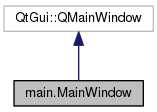
\includegraphics[width=190pt]{classmain_1_1_main_window__inherit__graph}
\end{center}
\end{figure}


Collaboration diagram for main.\-Main\-Window\-:\nopagebreak
\begin{figure}[H]
\begin{center}
\leavevmode
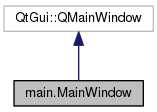
\includegraphics[width=190pt]{classmain_1_1_main_window__coll__graph}
\end{center}
\end{figure}
\subsubsection*{Public Member Functions}
\begin{DoxyCompactItemize}
\item 
def \hyperlink{classmain_1_1_main_window_afe60362fc3324bc53b3d0adc171cbc50}{\-\_\-\-\_\-init\-\_\-\-\_\-}
\begin{DoxyCompactList}\small\item\em Configures initial settings of the window. \end{DoxyCompactList}\item 
def \hyperlink{classmain_1_1_main_window_a2472e07b27a09bae26c1c064192cc7a0}{start}
\begin{DoxyCompactList}\small\item\em Executed when pressing Start Buttton. \end{DoxyCompactList}\item 
def \hyperlink{classmain_1_1_main_window_ac92cdbf6322bf71a1222ac4be72bb6c0}{update\-Data}
\begin{DoxyCompactList}\small\item\em Executed every time new data is adquired. \end{DoxyCompactList}\item 
\hypertarget{classmain_1_1_main_window_ae9e3c6d5509ddfa334a8c227565e6802}{def {\bfseries update\-Activity}}\label{classmain_1_1_main_window_ae9e3c6d5509ddfa334a8c227565e6802}

\item 
def \hyperlink{classmain_1_1_main_window_a758087e2cfebe24205f39e60d7b66840}{update\-Plot}
\begin{DoxyCompactList}\small\item\em Executed every 20 ms for updating plot. \end{DoxyCompactList}\item 
def \hyperlink{classmain_1_1_main_window_a15ec36789cc84d0227b1b6f680ed7b9b}{stop}
\begin{DoxyCompactList}\small\item\em Executed when Stop Button is pressed. \end{DoxyCompactList}\item 
def \hyperlink{classmain_1_1_main_window_a0f04f1f65afb676ff40644e3479ed429}{configure\-Plot}
\begin{DoxyCompactList}\small\item\em Axis configuration of a Py\-Qt\-Graph plot. \end{DoxyCompactList}\item 
def \hyperlink{classmain_1_1_main_window_a043c23015ff1c2e15228020289d2084b}{set\-U\-I\-Locked}
\begin{DoxyCompactList}\small\item\em Set the lock status of the U\-I elements. \end{DoxyCompactList}\item 
def \hyperlink{classmain_1_1_main_window_a3b91003f1660c283ae5061f3f228a7e2}{get\-Ports}
\begin{DoxyCompactList}\small\item\em Gets avaliable serial ports on the system. \end{DoxyCompactList}\item 
def \hyperlink{classmain_1_1_main_window_a6133369df2df9755fa172a60efc7239f}{reset\-Data}
\begin{DoxyCompactList}\small\item\em Clear data buffers for plotting. \end{DoxyCompactList}\item 
\hypertarget{classmain_1_1_main_window_aadf0b01331836efbc9cb5170f0f11085}{def {\bfseries start\-Cube}}\label{classmain_1_1_main_window_aadf0b01331836efbc9cb5170f0f11085}

\end{DoxyCompactItemize}
\subsubsection*{Public Attributes}
\begin{DoxyCompactItemize}
\item 
\hypertarget{classmain_1_1_main_window_ad4a5b9271a2213e10f7117bfa4f230f1}{{\bfseries ui}}\label{classmain_1_1_main_window_ad4a5b9271a2213e10f7117bfa4f230f1}

\item 
\hyperlink{classmain_1_1_main_window_ac830383d366fc669473cc4d94ab64efb}{timer}
\begin{DoxyCompactList}\small\item\em Reference update plot timer. \end{DoxyCompactList}\item 
\hypertarget{classmain_1_1_main_window_a4f2e2eac4efccf363c3b99c41ad14c48}{\hyperlink{classmain_1_1_main_window_a4f2e2eac4efccf363c3b99c41ad14c48}{timer\-Activity}}\label{classmain_1_1_main_window_a4f2e2eac4efccf363c3b99c41ad14c48}

\begin{DoxyCompactList}\small\item\em Qt4 timer for activity. \end{DoxyCompactList}\item 
\hyperlink{classmain_1_1_main_window_af7e14bdf821dcadf59ff9a25fdedacc6}{data}
\begin{DoxyCompactList}\small\item\em Reference for the Threaded serial adquisition. \end{DoxyCompactList}\item 
\hypertarget{classmain_1_1_main_window_aa93b2cedd13107177781d0044d78e8a0}{\hyperlink{classmain_1_1_main_window_aa93b2cedd13107177781d0044d78e8a0}{cube}}\label{classmain_1_1_main_window_aa93b2cedd13107177781d0044d78e8a0}

\begin{DoxyCompactList}\small\item\em Register the data object with the cube. \end{DoxyCompactList}\item 
\hypertarget{classmain_1_1_main_window_ac61cc125fc2941916e357bb8219a16ef}{\hyperlink{classmain_1_1_main_window_ac61cc125fc2941916e357bb8219a16ef}{csv}}\label{classmain_1_1_main_window_ac61cc125fc2941916e357bb8219a16ef}

\begin{DoxyCompactList}\small\item\em export data \end{DoxyCompactList}\item 
\hyperlink{classmain_1_1_main_window_a79bfc498bc7afae5335f0afa0457424c}{activity}
\begin{DoxyCompactList}\small\item\em Reference for the activity detection algorithm. \end{DoxyCompactList}\item 
\hyperlink{classmain_1_1_main_window_ac77d273e1ae89b15533af18cd3501efa}{fall}
\begin{DoxyCompactList}\small\item\em Reference for the fall detection algorithm. \end{DoxyCompactList}\item 
\hypertarget{classmain_1_1_main_window_a3cff3a6070c66ac5b036f882101c4e6c}{\hyperlink{classmain_1_1_main_window_a3cff3a6070c66ac5b036f882101c4e6c}{posture}}\label{classmain_1_1_main_window_a3cff3a6070c66ac5b036f882101c4e6c}

\begin{DoxyCompactList}\small\item\em Reference for. \end{DoxyCompactList}\item 
\hyperlink{classmain_1_1_main_window_a4bc63f3f953ad9110ea895e0b277e263}{A\-X}
\begin{DoxyCompactList}\small\item\em Buffer for Acceleration in X axis. \end{DoxyCompactList}\item 
\hyperlink{classmain_1_1_main_window_a0dd8435606fc6f9398de1c3759a5253e}{A\-Y}
\begin{DoxyCompactList}\small\item\em Buffer for Acceleration in Y axis. \end{DoxyCompactList}\item 
\hyperlink{classmain_1_1_main_window_aab50e3554ab90b750539200250578e0b}{A\-Z}
\begin{DoxyCompactList}\small\item\em Buffer for Acceleration in Z axis. \end{DoxyCompactList}\item 
\hyperlink{classmain_1_1_main_window_af9250994236464e4aa37faf090fa52b8}{G\-X}
\begin{DoxyCompactList}\small\item\em Buffer for Angular Velocity in X axis. \end{DoxyCompactList}\item 
\hyperlink{classmain_1_1_main_window_af19db177442479dc778051475277ee8b}{G\-Y}
\begin{DoxyCompactList}\small\item\em Buffer for Angular Velocity in Y axis. \end{DoxyCompactList}\item 
\hyperlink{classmain_1_1_main_window_aa03dbf9da18079ab07a57ebf5e523b58}{G\-Z}
\begin{DoxyCompactList}\small\item\em Buffer for Angular Velocity in Z axis. \end{DoxyCompactList}\item 
\hyperlink{classmain_1_1_main_window_a6ab8008a1a68f64ee8b6598a98654812}{M\-X}
\begin{DoxyCompactList}\small\item\em Buffer for Magnetic field in X axis. \end{DoxyCompactList}\item 
\hyperlink{classmain_1_1_main_window_aba40307f35350f664481c72b034e7bf8}{M\-Y}
\begin{DoxyCompactList}\small\item\em Buffer for Magnetic field in Y axis. \end{DoxyCompactList}\item 
\hyperlink{classmain_1_1_main_window_a3f1d2bc16eb2b7a565f2784e4741be7b}{M\-Z}
\begin{DoxyCompactList}\small\item\em Buffer for Magnetic field in Z axis. \end{DoxyCompactList}\item 
\hyperlink{classmain_1_1_main_window_a7b804cc35c413c631e3bb870bc123232}{Y}
\begin{DoxyCompactList}\small\item\em Buffer for Euler angles in X axis (Yaw) \end{DoxyCompactList}\item 
\hyperlink{classmain_1_1_main_window_a9000507d15f50881c7cfbd1d562e0feb}{P}
\begin{DoxyCompactList}\small\item\em Buffer for Euler angles in Y axis (Pitch) \end{DoxyCompactList}\item 
\hyperlink{classmain_1_1_main_window_a5a2a696186b46f2c1ab6d843781717bb}{R}
\begin{DoxyCompactList}\small\item\em Buffer for Euler angles in Z axis (Roll) \end{DoxyCompactList}\item 
\hyperlink{classmain_1_1_main_window_a7a3bc2d61217962905847f0badb89385}{Y2}
\begin{DoxyCompactList}\small\item\em Buffer for Euler angles in X axis (Yaw) \end{DoxyCompactList}\item 
\hyperlink{classmain_1_1_main_window_a27dae11aa90ae75ad58556b5f872d05e}{P2}
\begin{DoxyCompactList}\small\item\em Buffer for Euler angles in Y axis (Pitch) \end{DoxyCompactList}\item 
\hyperlink{classmain_1_1_main_window_a1a7ef29e7427ad606b2aacd8e1993e66}{R2}
\begin{DoxyCompactList}\small\item\em Buffer for Euler angles in Z axis (Roll) \end{DoxyCompactList}\item 
\hyperlink{classmain_1_1_main_window_a689266200b7e4956e7e5c0fa52093dda}{L\-A\-X}
\begin{DoxyCompactList}\small\item\em Buffer for Linear Acceleration in X axis. \end{DoxyCompactList}\item 
\hyperlink{classmain_1_1_main_window_a6da1afdc121f84b6eb02beb0db52049a}{L\-A\-Y}
\begin{DoxyCompactList}\small\item\em Buffer for Linear Acceleration in Y axis. \end{DoxyCompactList}\item 
\hyperlink{classmain_1_1_main_window_af8a0057e50f3209b22653600a36db22a}{L\-A\-Z}
\begin{DoxyCompactList}\small\item\em Buffer for Linear Acceleration in Z axis. \end{DoxyCompactList}\item 
\hyperlink{classmain_1_1_main_window_ac295e7edaa6b0c00592ea04ecd01ce78}{P\-O\-S}
\begin{DoxyCompactList}\small\item\em Indicates the current index for storing data in the buffers. \end{DoxyCompactList}\end{DoxyCompactItemize}


\subsubsection{Detailed Description}
Managing and plotting adquired data. 


\begin{DoxyParams}{Parameters}
{\em Qt\-Gui.\-Q\-Main\-Window} & Qt4 Main Window reference \\
\hline
\end{DoxyParams}


\subsubsection{Constructor \& Destructor Documentation}
\hypertarget{classmain_1_1_main_window_afe60362fc3324bc53b3d0adc171cbc50}{\index{main\-::\-Main\-Window@{main\-::\-Main\-Window}!\-\_\-\-\_\-init\-\_\-\-\_\-@{\-\_\-\-\_\-init\-\_\-\-\_\-}}
\index{\-\_\-\-\_\-init\-\_\-\-\_\-@{\-\_\-\-\_\-init\-\_\-\-\_\-}!main::MainWindow@{main\-::\-Main\-Window}}
\paragraph[{\-\_\-\-\_\-init\-\_\-\-\_\-}]{\setlength{\rightskip}{0pt plus 5cm}def main.\-Main\-Window.\-\_\-\-\_\-init\-\_\-\-\_\- (
\begin{DoxyParamCaption}
\item[{}]{self}
\end{DoxyParamCaption}
)}}\label{classmain_1_1_main_window_afe60362fc3324bc53b3d0adc171cbc50}


Configures initial settings of the window. 

Initialize data, plots, imported functions and timers 

\subsubsection{Member Function Documentation}
\hypertarget{classmain_1_1_main_window_a0f04f1f65afb676ff40644e3479ed429}{\index{main\-::\-Main\-Window@{main\-::\-Main\-Window}!configure\-Plot@{configure\-Plot}}
\index{configure\-Plot@{configure\-Plot}!main::MainWindow@{main\-::\-Main\-Window}}
\paragraph[{configure\-Plot}]{\setlength{\rightskip}{0pt plus 5cm}def main.\-Main\-Window.\-configure\-Plot (
\begin{DoxyParamCaption}
\item[{}]{self, }
\item[{}]{plot, }
\item[{}]{Range, }
\item[{}]{title, }
\item[{}]{unit}
\end{DoxyParamCaption}
)}}\label{classmain_1_1_main_window_a0f04f1f65afb676ff40644e3479ed429}


Axis configuration of a Py\-Qt\-Graph plot. 

Stops data threads, timers and unlocks U\-I. 
\begin{DoxyParams}{Parameters}
{\em self} & The object pointer. \\
\hline
{\em plot} & The reference to the plot to be configured \\
\hline
{\em Range} & The range (+/-\/) for the Y axis of the plot \\
\hline
{\em title} & The title of the plot \\
\hline
{\em unit} & The measurement unit for the plot (auto-\/scaled) \\
\hline
\end{DoxyParams}
\hypertarget{classmain_1_1_main_window_a3b91003f1660c283ae5061f3f228a7e2}{\index{main\-::\-Main\-Window@{main\-::\-Main\-Window}!get\-Ports@{get\-Ports}}
\index{get\-Ports@{get\-Ports}!main::MainWindow@{main\-::\-Main\-Window}}
\paragraph[{get\-Ports}]{\setlength{\rightskip}{0pt plus 5cm}def main.\-Main\-Window.\-get\-Ports (
\begin{DoxyParamCaption}
\item[{}]{self}
\end{DoxyParamCaption}
)}}\label{classmain_1_1_main_window_a3b91003f1660c283ae5061f3f228a7e2}


Gets avaliable serial ports on the system. 

Search trough all avaliable serial ports (virtuals included) and lists only those who have a connection avaliable. 
\begin{DoxyParams}{Parameters}
{\em self} & The object pointer. \\
\hline
\end{DoxyParams}

\begin{DoxyRetVals}{Return values}
{\em port\-List} & list with the serial ports routes \\
\hline
\end{DoxyRetVals}
\hypertarget{classmain_1_1_main_window_a6133369df2df9755fa172a60efc7239f}{\index{main\-::\-Main\-Window@{main\-::\-Main\-Window}!reset\-Data@{reset\-Data}}
\index{reset\-Data@{reset\-Data}!main::MainWindow@{main\-::\-Main\-Window}}
\paragraph[{reset\-Data}]{\setlength{\rightskip}{0pt plus 5cm}def main.\-Main\-Window.\-reset\-Data (
\begin{DoxyParamCaption}
\item[{}]{self}
\end{DoxyParamCaption}
)}}\label{classmain_1_1_main_window_a6133369df2df9755fa172a60efc7239f}


Clear data buffers for plotting. 

Fill with zeroes all data buffers used for plotting and position the data.

Size of the buffers can be changed by the class variable W\-I\-N\-D\-O\-W 
\begin{DoxyParams}{Parameters}
{\em self} & The object pointer. \\
\hline
\end{DoxyParams}
\hypertarget{classmain_1_1_main_window_a043c23015ff1c2e15228020289d2084b}{\index{main\-::\-Main\-Window@{main\-::\-Main\-Window}!set\-U\-I\-Locked@{set\-U\-I\-Locked}}
\index{set\-U\-I\-Locked@{set\-U\-I\-Locked}!main::MainWindow@{main\-::\-Main\-Window}}
\paragraph[{set\-U\-I\-Locked}]{\setlength{\rightskip}{0pt plus 5cm}def main.\-Main\-Window.\-set\-U\-I\-Locked (
\begin{DoxyParamCaption}
\item[{}]{self, }
\item[{}]{bool\-\_\-}
\end{DoxyParamCaption}
)}}\label{classmain_1_1_main_window_a043c23015ff1c2e15228020289d2084b}


Set the lock status of the U\-I elements. 

Enables or disables U\-I elements of the window. Executed during adquisition, blocks U\-I elements to only enable the Stop button and disable configuration U\-I elements.


\begin{DoxyItemize}
\item if {\ttfamily bool\-\_\-} = {\bfseries T\-R\-U\-E\-:} allows configuration of the adquisition
\item if {\ttfamily bool\-\_\-} = {\bfseries F\-A\-L\-S\-E\-:} disables configuratin of the adquisition 
\begin{DoxyParams}{Parameters}
{\em self} & The object pointer. \\
\hline
{\em bool\-\_\-} & The status of the U\-I \\
\hline
\end{DoxyParams}

\end{DoxyItemize}\hypertarget{classmain_1_1_main_window_a2472e07b27a09bae26c1c064192cc7a0}{\index{main\-::\-Main\-Window@{main\-::\-Main\-Window}!start@{start}}
\index{start@{start}!main::MainWindow@{main\-::\-Main\-Window}}
\paragraph[{start}]{\setlength{\rightskip}{0pt plus 5cm}def main.\-Main\-Window.\-start (
\begin{DoxyParamCaption}
\item[{}]{self}
\end{DoxyParamCaption}
)}}\label{classmain_1_1_main_window_a2472e07b27a09bae26c1c064192cc7a0}


Executed when pressing Start Buttton. 

Starts data adquisition and timers, blocking the U\-I elements 
\begin{DoxyParams}{Parameters}
{\em self} & The object pointer. \\
\hline
\end{DoxyParams}
\hypertarget{classmain_1_1_main_window_a15ec36789cc84d0227b1b6f680ed7b9b}{\index{main\-::\-Main\-Window@{main\-::\-Main\-Window}!stop@{stop}}
\index{stop@{stop}!main::MainWindow@{main\-::\-Main\-Window}}
\paragraph[{stop}]{\setlength{\rightskip}{0pt plus 5cm}def main.\-Main\-Window.\-stop (
\begin{DoxyParamCaption}
\item[{}]{self}
\end{DoxyParamCaption}
)}}\label{classmain_1_1_main_window_a15ec36789cc84d0227b1b6f680ed7b9b}


Executed when Stop Button is pressed. 

Stops data threads, timers and unlocks U\-I. 
\begin{DoxyParams}{Parameters}
{\em self} & The object pointer. \\
\hline
\end{DoxyParams}
\hypertarget{classmain_1_1_main_window_ac92cdbf6322bf71a1222ac4be72bb6c0}{\index{main\-::\-Main\-Window@{main\-::\-Main\-Window}!update\-Data@{update\-Data}}
\index{update\-Data@{update\-Data}!main::MainWindow@{main\-::\-Main\-Window}}
\paragraph[{update\-Data}]{\setlength{\rightskip}{0pt plus 5cm}def main.\-Main\-Window.\-update\-Data (
\begin{DoxyParamCaption}
\item[{}]{self}
\end{DoxyParamCaption}
)}}\label{classmain_1_1_main_window_ac92cdbf6322bf71a1222ac4be72bb6c0}


Executed every time new data is adquired. 

Executed by serial\-Thread\-\_\-\-M\-P\-U9150 with Q\-T4 Signal 
\begin{DoxyParams}{Parameters}
{\em self} & The object pointer. \\
\hline
\end{DoxyParams}
\hypertarget{classmain_1_1_main_window_a758087e2cfebe24205f39e60d7b66840}{\index{main\-::\-Main\-Window@{main\-::\-Main\-Window}!update\-Plot@{update\-Plot}}
\index{update\-Plot@{update\-Plot}!main::MainWindow@{main\-::\-Main\-Window}}
\paragraph[{update\-Plot}]{\setlength{\rightskip}{0pt plus 5cm}def main.\-Main\-Window.\-update\-Plot (
\begin{DoxyParamCaption}
\item[{}]{self}
\end{DoxyParamCaption}
)}}\label{classmain_1_1_main_window_a758087e2cfebe24205f39e60d7b66840}


Executed every 20 ms for updating plot. 

Executed by Qt\-Timer every 20 ms after pressed start button. Stops and reset timer when stop button is pressed. 
\begin{DoxyParams}{Parameters}
{\em self} & The object pointers \\
\hline
\end{DoxyParams}


\subsubsection{Member Data Documentation}
\hypertarget{classmain_1_1_main_window_a79bfc498bc7afae5335f0afa0457424c}{\index{main\-::\-Main\-Window@{main\-::\-Main\-Window}!activity@{activity}}
\index{activity@{activity}!main::MainWindow@{main\-::\-Main\-Window}}
\paragraph[{activity}]{\setlength{\rightskip}{0pt plus 5cm}main.\-Main\-Window.\-activity}}\label{classmain_1_1_main_window_a79bfc498bc7afae5335f0afa0457424c}


Reference for the activity detection algorithm. 

Activity detection algorithm propossed by Dr. Pablo Reyes \hypertarget{classmain_1_1_main_window_a4bc63f3f953ad9110ea895e0b277e263}{\index{main\-::\-Main\-Window@{main\-::\-Main\-Window}!A\-X@{A\-X}}
\index{A\-X@{A\-X}!main::MainWindow@{main\-::\-Main\-Window}}
\paragraph[{A\-X}]{\setlength{\rightskip}{0pt plus 5cm}main.\-Main\-Window.\-A\-X}}\label{classmain_1_1_main_window_a4bc63f3f953ad9110ea895e0b277e263}


Buffer for Acceleration in X axis. 

Acceleration in g (gravity) \hypertarget{classmain_1_1_main_window_a0dd8435606fc6f9398de1c3759a5253e}{\index{main\-::\-Main\-Window@{main\-::\-Main\-Window}!A\-Y@{A\-Y}}
\index{A\-Y@{A\-Y}!main::MainWindow@{main\-::\-Main\-Window}}
\paragraph[{A\-Y}]{\setlength{\rightskip}{0pt plus 5cm}main.\-Main\-Window.\-A\-Y}}\label{classmain_1_1_main_window_a0dd8435606fc6f9398de1c3759a5253e}


Buffer for Acceleration in Y axis. 

Acceleration in g (gravity) \hypertarget{classmain_1_1_main_window_aab50e3554ab90b750539200250578e0b}{\index{main\-::\-Main\-Window@{main\-::\-Main\-Window}!A\-Z@{A\-Z}}
\index{A\-Z@{A\-Z}!main::MainWindow@{main\-::\-Main\-Window}}
\paragraph[{A\-Z}]{\setlength{\rightskip}{0pt plus 5cm}main.\-Main\-Window.\-A\-Z}}\label{classmain_1_1_main_window_aab50e3554ab90b750539200250578e0b}


Buffer for Acceleration in Z axis. 

Acceleration in g (gravity) \hypertarget{classmain_1_1_main_window_af7e14bdf821dcadf59ff9a25fdedacc6}{\index{main\-::\-Main\-Window@{main\-::\-Main\-Window}!data@{data}}
\index{data@{data}!main::MainWindow@{main\-::\-Main\-Window}}
\paragraph[{data}]{\setlength{\rightskip}{0pt plus 5cm}main.\-Main\-Window.\-data}}\label{classmain_1_1_main_window_af7e14bdf821dcadf59ff9a25fdedacc6}


Reference for the Threaded serial adquisition. 

Threaded adquisition for a serial device with interrupts using Qt4 signals \hypertarget{classmain_1_1_main_window_ac77d273e1ae89b15533af18cd3501efa}{\index{main\-::\-Main\-Window@{main\-::\-Main\-Window}!fall@{fall}}
\index{fall@{fall}!main::MainWindow@{main\-::\-Main\-Window}}
\paragraph[{fall}]{\setlength{\rightskip}{0pt plus 5cm}main.\-Main\-Window.\-fall}}\label{classmain_1_1_main_window_ac77d273e1ae89b15533af18cd3501efa}


Reference for the fall detection algorithm. 

Fall detection algorithm propossed by Dr. Pablo Reyes \hypertarget{classmain_1_1_main_window_af9250994236464e4aa37faf090fa52b8}{\index{main\-::\-Main\-Window@{main\-::\-Main\-Window}!G\-X@{G\-X}}
\index{G\-X@{G\-X}!main::MainWindow@{main\-::\-Main\-Window}}
\paragraph[{G\-X}]{\setlength{\rightskip}{0pt plus 5cm}main.\-Main\-Window.\-G\-X}}\label{classmain_1_1_main_window_af9250994236464e4aa37faf090fa52b8}


Buffer for Angular Velocity in X axis. 

Angular Velocity in degrees/second \hypertarget{classmain_1_1_main_window_af19db177442479dc778051475277ee8b}{\index{main\-::\-Main\-Window@{main\-::\-Main\-Window}!G\-Y@{G\-Y}}
\index{G\-Y@{G\-Y}!main::MainWindow@{main\-::\-Main\-Window}}
\paragraph[{G\-Y}]{\setlength{\rightskip}{0pt plus 5cm}main.\-Main\-Window.\-G\-Y}}\label{classmain_1_1_main_window_af19db177442479dc778051475277ee8b}


Buffer for Angular Velocity in Y axis. 

Angular Velocity in degrees/second \hypertarget{classmain_1_1_main_window_aa03dbf9da18079ab07a57ebf5e523b58}{\index{main\-::\-Main\-Window@{main\-::\-Main\-Window}!G\-Z@{G\-Z}}
\index{G\-Z@{G\-Z}!main::MainWindow@{main\-::\-Main\-Window}}
\paragraph[{G\-Z}]{\setlength{\rightskip}{0pt plus 5cm}main.\-Main\-Window.\-G\-Z}}\label{classmain_1_1_main_window_aa03dbf9da18079ab07a57ebf5e523b58}


Buffer for Angular Velocity in Z axis. 

Angular Velocity in degrees/second \hypertarget{classmain_1_1_main_window_a689266200b7e4956e7e5c0fa52093dda}{\index{main\-::\-Main\-Window@{main\-::\-Main\-Window}!L\-A\-X@{L\-A\-X}}
\index{L\-A\-X@{L\-A\-X}!main::MainWindow@{main\-::\-Main\-Window}}
\paragraph[{L\-A\-X}]{\setlength{\rightskip}{0pt plus 5cm}main.\-Main\-Window.\-L\-A\-X}}\label{classmain_1_1_main_window_a689266200b7e4956e7e5c0fa52093dda}


Buffer for Linear Acceleration in X axis. 

Acceleration in g (gravity). The 9\-D\-O\-F sensor fusion algorithm allows to estimate the expected gravity coordinates and dinamically delete it from the measured acceleration, allowing the gravity compensated linear acceleration \hypertarget{classmain_1_1_main_window_a6da1afdc121f84b6eb02beb0db52049a}{\index{main\-::\-Main\-Window@{main\-::\-Main\-Window}!L\-A\-Y@{L\-A\-Y}}
\index{L\-A\-Y@{L\-A\-Y}!main::MainWindow@{main\-::\-Main\-Window}}
\paragraph[{L\-A\-Y}]{\setlength{\rightskip}{0pt plus 5cm}main.\-Main\-Window.\-L\-A\-Y}}\label{classmain_1_1_main_window_a6da1afdc121f84b6eb02beb0db52049a}


Buffer for Linear Acceleration in Y axis. 

Acceleration in g (gravity). The 9\-D\-O\-F sensor fusion algorithm allows to estimate the expected gravity coordinates and dinamically delete it from the measured acceleration, allowing the gravity compensated linear acceleration \hypertarget{classmain_1_1_main_window_af8a0057e50f3209b22653600a36db22a}{\index{main\-::\-Main\-Window@{main\-::\-Main\-Window}!L\-A\-Z@{L\-A\-Z}}
\index{L\-A\-Z@{L\-A\-Z}!main::MainWindow@{main\-::\-Main\-Window}}
\paragraph[{L\-A\-Z}]{\setlength{\rightskip}{0pt plus 5cm}main.\-Main\-Window.\-L\-A\-Z}}\label{classmain_1_1_main_window_af8a0057e50f3209b22653600a36db22a}


Buffer for Linear Acceleration in Z axis. 

Acceleration in g (gravity). The 9\-D\-O\-F sensor fusion algorithm allows to estimate the expected gravity coordinates and dinamically delete it from the measured acceleration, allowing the gravity compensated linear acceleration \hypertarget{classmain_1_1_main_window_a6ab8008a1a68f64ee8b6598a98654812}{\index{main\-::\-Main\-Window@{main\-::\-Main\-Window}!M\-X@{M\-X}}
\index{M\-X@{M\-X}!main::MainWindow@{main\-::\-Main\-Window}}
\paragraph[{M\-X}]{\setlength{\rightskip}{0pt plus 5cm}main.\-Main\-Window.\-M\-X}}\label{classmain_1_1_main_window_a6ab8008a1a68f64ee8b6598a98654812}


Buffer for Magnetic field in X axis. 

Magnetic field flux in Gauss (Gs) \hypertarget{classmain_1_1_main_window_aba40307f35350f664481c72b034e7bf8}{\index{main\-::\-Main\-Window@{main\-::\-Main\-Window}!M\-Y@{M\-Y}}
\index{M\-Y@{M\-Y}!main::MainWindow@{main\-::\-Main\-Window}}
\paragraph[{M\-Y}]{\setlength{\rightskip}{0pt plus 5cm}main.\-Main\-Window.\-M\-Y}}\label{classmain_1_1_main_window_aba40307f35350f664481c72b034e7bf8}


Buffer for Magnetic field in Y axis. 

Magnetic field flux in Gauss (Gs) \hypertarget{classmain_1_1_main_window_a3f1d2bc16eb2b7a565f2784e4741be7b}{\index{main\-::\-Main\-Window@{main\-::\-Main\-Window}!M\-Z@{M\-Z}}
\index{M\-Z@{M\-Z}!main::MainWindow@{main\-::\-Main\-Window}}
\paragraph[{M\-Z}]{\setlength{\rightskip}{0pt plus 5cm}main.\-Main\-Window.\-M\-Z}}\label{classmain_1_1_main_window_a3f1d2bc16eb2b7a565f2784e4741be7b}


Buffer for Magnetic field in Z axis. 

Magnetic field flux in Gauss (Gs) \hypertarget{classmain_1_1_main_window_a9000507d15f50881c7cfbd1d562e0feb}{\index{main\-::\-Main\-Window@{main\-::\-Main\-Window}!P@{P}}
\index{P@{P}!main::MainWindow@{main\-::\-Main\-Window}}
\paragraph[{P}]{\setlength{\rightskip}{0pt plus 5cm}main.\-Main\-Window.\-P}}\label{classmain_1_1_main_window_a9000507d15f50881c7cfbd1d562e0feb}


Buffer for Euler angles in Y axis (Pitch) 

Angles in degrees. Obtained directicly from the D\-M\-P of the M\-P\-U-\/9150 internal sensor fusion with 6\-D\-O\-F (Accelerometer + Gyroscope). \hypertarget{classmain_1_1_main_window_a27dae11aa90ae75ad58556b5f872d05e}{\index{main\-::\-Main\-Window@{main\-::\-Main\-Window}!P2@{P2}}
\index{P2@{P2}!main::MainWindow@{main\-::\-Main\-Window}}
\paragraph[{P2}]{\setlength{\rightskip}{0pt plus 5cm}main.\-Main\-Window.\-P2}}\label{classmain_1_1_main_window_a27dae11aa90ae75ad58556b5f872d05e}


Buffer for Euler angles in Y axis (Pitch) 

Angles in degrees. Obtained from the sensor fusion algorithm (9\-D\-O\-F) developed by Sebastian Madgwick and implemented by Fabio Varesano. \hypertarget{classmain_1_1_main_window_ac295e7edaa6b0c00592ea04ecd01ce78}{\index{main\-::\-Main\-Window@{main\-::\-Main\-Window}!P\-O\-S@{P\-O\-S}}
\index{P\-O\-S@{P\-O\-S}!main::MainWindow@{main\-::\-Main\-Window}}
\paragraph[{P\-O\-S}]{\setlength{\rightskip}{0pt plus 5cm}main.\-Main\-Window.\-P\-O\-S}}\label{classmain_1_1_main_window_ac295e7edaa6b0c00592ea04ecd01ce78}


Indicates the current index for storing data in the buffers. 

Updated and reseted by \hyperlink{classmain_1_1_main_window_ac92cdbf6322bf71a1222ac4be72bb6c0}{update\-Data} limits its count to W\-I\-N\-D\-O\-W variable \hypertarget{classmain_1_1_main_window_a5a2a696186b46f2c1ab6d843781717bb}{\index{main\-::\-Main\-Window@{main\-::\-Main\-Window}!R@{R}}
\index{R@{R}!main::MainWindow@{main\-::\-Main\-Window}}
\paragraph[{R}]{\setlength{\rightskip}{0pt plus 5cm}main.\-Main\-Window.\-R}}\label{classmain_1_1_main_window_a5a2a696186b46f2c1ab6d843781717bb}


Buffer for Euler angles in Z axis (Roll) 

Angles in degrees. Obtained directicly from the D\-M\-P of the M\-P\-U-\/9150 internal sensor fusion with 6\-D\-O\-F (Accelerometer + Gyroscope). \hypertarget{classmain_1_1_main_window_a1a7ef29e7427ad606b2aacd8e1993e66}{\index{main\-::\-Main\-Window@{main\-::\-Main\-Window}!R2@{R2}}
\index{R2@{R2}!main::MainWindow@{main\-::\-Main\-Window}}
\paragraph[{R2}]{\setlength{\rightskip}{0pt plus 5cm}main.\-Main\-Window.\-R2}}\label{classmain_1_1_main_window_a1a7ef29e7427ad606b2aacd8e1993e66}


Buffer for Euler angles in Z axis (Roll) 

Angles in degrees. Obtained from the sensor fusion algorithm (9\-D\-O\-F) developed by Sebastian Madgwick and implemented by Fabio Varesano. \hypertarget{classmain_1_1_main_window_ac830383d366fc669473cc4d94ab64efb}{\index{main\-::\-Main\-Window@{main\-::\-Main\-Window}!timer@{timer}}
\index{timer@{timer}!main::MainWindow@{main\-::\-Main\-Window}}
\paragraph[{timer}]{\setlength{\rightskip}{0pt plus 5cm}main.\-Main\-Window.\-timer}}\label{classmain_1_1_main_window_ac830383d366fc669473cc4d94ab64efb}


Reference update plot timer. 

Qt4 timer to trigger the  function \hypertarget{classmain_1_1_main_window_a7b804cc35c413c631e3bb870bc123232}{\index{main\-::\-Main\-Window@{main\-::\-Main\-Window}!Y@{Y}}
\index{Y@{Y}!main::MainWindow@{main\-::\-Main\-Window}}
\paragraph[{Y}]{\setlength{\rightskip}{0pt plus 5cm}main.\-Main\-Window.\-Y}}\label{classmain_1_1_main_window_a7b804cc35c413c631e3bb870bc123232}


Buffer for Euler angles in X axis (Yaw) 

Angles in degrees. Obtained directicly from the D\-M\-P of the M\-P\-U-\/9150 internal sensor fusion with 6\-D\-O\-F (Accelerometer + Gyroscope). \hypertarget{classmain_1_1_main_window_a7a3bc2d61217962905847f0badb89385}{\index{main\-::\-Main\-Window@{main\-::\-Main\-Window}!Y2@{Y2}}
\index{Y2@{Y2}!main::MainWindow@{main\-::\-Main\-Window}}
\paragraph[{Y2}]{\setlength{\rightskip}{0pt plus 5cm}main.\-Main\-Window.\-Y2}}\label{classmain_1_1_main_window_a7a3bc2d61217962905847f0badb89385}


Buffer for Euler angles in X axis (Yaw) 

Angles in degrees. Obtained from the sensor fusion algorithm (9\-D\-O\-F) developed by Sebastian Madgwick and implemented by Fabio Varesano. 

The documentation for this class was generated from the following file\-:\begin{DoxyCompactItemize}
\item 
I\-M\-U\-Graph/main.\-py\end{DoxyCompactItemize}

\hypertarget{classposture_1_1_posture}{\subsection{posture.\-Posture Class Reference}
\label{classposture_1_1_posture}\index{posture.\-Posture@{posture.\-Posture}}
}


\hyperlink{classposture_1_1_posture}{Posture} estimation based on accelerometer used as a compensated tilt sensor.  


\subsubsection*{Public Member Functions}
\begin{DoxyCompactItemize}
\item 
\hypertarget{classposture_1_1_posture_a83e447c26b71e109493860eb3157c409}{def \hyperlink{classposture_1_1_posture_a83e447c26b71e109493860eb3157c409}{\-\_\-\-\_\-init\-\_\-\-\_\-}}\label{classposture_1_1_posture_a83e447c26b71e109493860eb3157c409}

\begin{DoxyCompactList}\small\item\em Constructor. \end{DoxyCompactList}\item 
def \hyperlink{classposture_1_1_posture_aaf778c81f563ea4eae7a46227085fb2b}{offset}
\begin{DoxyCompactList}\small\item\em Determinates the offset in the accelerometer. \end{DoxyCompactList}\item 
def \hyperlink{classposture_1_1_posture_aaf817d25ff93679ced24d2786e0944e2}{compensated\-Tilt}
\begin{DoxyCompactList}\small\item\em Compesated tilt. \end{DoxyCompactList}\item 
def \hyperlink{classposture_1_1_posture_a6548993924c0cbea896f6448d24491b8}{normalize}
\begin{DoxyCompactList}\small\item\em Normalizes de values of the gravity. \end{DoxyCompactList}\item 
def \hyperlink{classposture_1_1_posture_a301e34481371c95c06434f89b2a6ad39}{mean}
\begin{DoxyCompactList}\small\item\em Average of a list of values. \end{DoxyCompactList}\item 
def \hyperlink{classposture_1_1_posture_ad9bc6d06a96d33b488094a295a4c3f4c}{reset\-Buffers}
\begin{DoxyCompactList}\small\item\em Clean buffers. \end{DoxyCompactList}\item 
def \hyperlink{classposture_1_1_posture_ae8c17334701e824d29ede0fd6a8baa78}{get\-Tilt}
\begin{DoxyCompactList}\small\item\em Getter for the tilt values. \end{DoxyCompactList}\end{DoxyCompactItemize}
\subsubsection*{Public Attributes}
\begin{DoxyCompactItemize}
\item 
\hypertarget{classposture_1_1_posture_a8007dea4830a05937eeed93a734e5f91}{{\bfseries g}}\label{classposture_1_1_posture_a8007dea4830a05937eeed93a734e5f91}

\item 
\hypertarget{classposture_1_1_posture_aedef5377473c2e20d16c88440e514763}{{\bfseries angle\-\_\-frontal}}\label{classposture_1_1_posture_aedef5377473c2e20d16c88440e514763}

\item 
\hypertarget{classposture_1_1_posture_a145e040bf762b3169e8157665b31e3f0}{{\bfseries angle\-\_\-lateral}}\label{classposture_1_1_posture_a145e040bf762b3169e8157665b31e3f0}

\item 
\hypertarget{classposture_1_1_posture_abdd37b491d8194f255c0017dcd32b6a6}{{\bfseries X}}\label{classposture_1_1_posture_abdd37b491d8194f255c0017dcd32b6a6}

\item 
\hypertarget{classposture_1_1_posture_a267afdbb1a17dba6c619d3ac2d7a9892}{{\bfseries Y}}\label{classposture_1_1_posture_a267afdbb1a17dba6c619d3ac2d7a9892}

\item 
\hypertarget{classposture_1_1_posture_aa251677d3dcf44e8c7c37007bcbb29d8}{{\bfseries Z}}\label{classposture_1_1_posture_aa251677d3dcf44e8c7c37007bcbb29d8}

\end{DoxyCompactItemize}
\subsubsection*{Static Public Attributes}
\begin{DoxyCompactItemize}
\item 
\hypertarget{classposture_1_1_posture_a8c705a4aac70c0f0de40cdb9bb816516}{int {\bfseries std} = .\-05}\label{classposture_1_1_posture_a8c705a4aac70c0f0de40cdb9bb816516}

\item 
\hypertarget{classposture_1_1_posture_af09f6fce94fafc627216b8a7529d39d7}{list {\bfseries g} = \mbox{[}0\mbox{]}}\label{classposture_1_1_posture_af09f6fce94fafc627216b8a7529d39d7}

\end{DoxyCompactItemize}


\subsubsection{Detailed Description}
\hyperlink{classposture_1_1_posture}{Posture} estimation based on accelerometer used as a compensated tilt sensor. 

The algoritm calculates the offset due to earth's gravity in the accelerometer axis, provided no other accelerations or forces affects the accelerometer.

The algorithm then determinates the tilt componsated with the estimated position of the gravity, to ensure the measurements are always equals in the coordinates of the accelerometer. \begin{DoxyAuthor}{Author}
Sebastian Sepulveda 
\end{DoxyAuthor}


\subsubsection{Member Function Documentation}
\hypertarget{classposture_1_1_posture_aaf817d25ff93679ced24d2786e0944e2}{\index{posture\-::\-Posture@{posture\-::\-Posture}!compensated\-Tilt@{compensated\-Tilt}}
\index{compensated\-Tilt@{compensated\-Tilt}!posture::Posture@{posture\-::\-Posture}}
\paragraph[{compensated\-Tilt}]{\setlength{\rightskip}{0pt plus 5cm}def posture.\-Posture.\-compensated\-Tilt (
\begin{DoxyParamCaption}
\item[{}]{self, }
\item[{}]{x, }
\item[{}]{y, }
\item[{}]{z}
\end{DoxyParamCaption}
)}}\label{classposture_1_1_posture_aaf817d25ff93679ced24d2786e0944e2}


Compesated tilt. 

Using the data generated by \hyperlink{classposture_1_1_posture_aaf778c81f563ea4eae7a46227085fb2b}{offset}, modifies axis values gatered so the tilt is always measured properly, based on this considerations\-:


\begin{DoxyItemize}
\item The earth's gravity is aligned with the z axis (axis pointing in direction of the earth's gravity)
\item The Y axis points to the front of the user
\item The X axis points to the right of the user
\end{DoxyItemize}

With this considerations, the rest of the modifications based on the displacement of the earth's gravity are reorder to calculate the tilt alway in reference to the earth's gravity 
\begin{DoxyParams}{Parameters}
{\em self} & The object pointer. \\
\hline
{\em x} & Acceleration in the x axis, in g \\
\hline
{\em y} & Acceleration in the y axis, in g \\
\hline
{\em z} & Acceleration in the z axis, in g \\
\hline
\end{DoxyParams}
\hypertarget{classposture_1_1_posture_ae8c17334701e824d29ede0fd6a8baa78}{\index{posture\-::\-Posture@{posture\-::\-Posture}!get\-Tilt@{get\-Tilt}}
\index{get\-Tilt@{get\-Tilt}!posture::Posture@{posture\-::\-Posture}}
\paragraph[{get\-Tilt}]{\setlength{\rightskip}{0pt plus 5cm}def posture.\-Posture.\-get\-Tilt (
\begin{DoxyParamCaption}
\item[{}]{self, }
\item[{}]{x, }
\item[{}]{y, }
\item[{}]{z}
\end{DoxyParamCaption}
)}}\label{classposture_1_1_posture_ae8c17334701e824d29ede0fd6a8baa78}


Getter for the tilt values. 


\begin{DoxyParams}{Parameters}
{\em self} & The object pointer. \\
\hline
{\em x} & Acceleration in the x axis, in g \\
\hline
{\em y} & Acceleration in the y axis, in g \\
\hline
{\em z} & Acceleration in the z axis, in g \\
\hline
\end{DoxyParams}
\begin{DoxyReturn}{Returns}
A list with 2 elements
\begin{DoxyItemize}
\item {\bfseries 1st} Position show the tilt inclination.
\begin{DoxyItemize}
\item {\bfseries Positive} values means front inclination
\item {\bfseries Negative} values means backwards inclination
\end{DoxyItemize}
\item {\bfseries 2nd} Position show the tilt inclination.
\begin{DoxyItemize}
\item {\bfseries Positive} values means right inclination
\item {\bfseries Negative} values means left inclination 
\end{DoxyItemize}
\end{DoxyItemize}
\end{DoxyReturn}
\hypertarget{classposture_1_1_posture_a301e34481371c95c06434f89b2a6ad39}{\index{posture\-::\-Posture@{posture\-::\-Posture}!mean@{mean}}
\index{mean@{mean}!posture::Posture@{posture\-::\-Posture}}
\paragraph[{mean}]{\setlength{\rightskip}{0pt plus 5cm}def posture.\-Posture.\-mean (
\begin{DoxyParamCaption}
\item[{}]{self, }
\item[{}]{list\-\_\-}
\end{DoxyParamCaption}
)}}\label{classposture_1_1_posture_a301e34481371c95c06434f89b2a6ad39}


Average of a list of values. 


\begin{DoxyParams}{Parameters}
{\em self} & The object pointer. \\
\hline
{\em list\-\_\-} & list with values \\
\hline
\end{DoxyParams}
\begin{DoxyReturn}{Returns}
Average of the List 
\end{DoxyReturn}
\hypertarget{classposture_1_1_posture_a6548993924c0cbea896f6448d24491b8}{\index{posture\-::\-Posture@{posture\-::\-Posture}!normalize@{normalize}}
\index{normalize@{normalize}!posture::Posture@{posture\-::\-Posture}}
\paragraph[{normalize}]{\setlength{\rightskip}{0pt plus 5cm}def posture.\-Posture.\-normalize (
\begin{DoxyParamCaption}
\item[{}]{self, }
\item[{}]{value}
\end{DoxyParamCaption}
)}}\label{classposture_1_1_posture_a6548993924c0cbea896f6448d24491b8}


Normalizes de values of the gravity. 

Normalizes values in 3 ranges, using the std as desviation from the expected values 
\begin{DoxyParams}{Parameters}
{\em self} & The object pointer. \\
\hline
{\em value} & Value to be normalized \\
\hline
\end{DoxyParams}
\begin{DoxyReturn}{Returns}
normalized values
\begin{DoxyItemize}
\item {\bfseries 1} if the gravity points in the direction of the axis
\item {\bfseries 0} if the gravity was not detected in the axis
\item {\bfseries 1} if the gravity points in the opposite direction of the axis 
\end{DoxyItemize}
\end{DoxyReturn}
\hypertarget{classposture_1_1_posture_aaf778c81f563ea4eae7a46227085fb2b}{\index{posture\-::\-Posture@{posture\-::\-Posture}!offset@{offset}}
\index{offset@{offset}!posture::Posture@{posture\-::\-Posture}}
\paragraph[{offset}]{\setlength{\rightskip}{0pt plus 5cm}def posture.\-Posture.\-offset (
\begin{DoxyParamCaption}
\item[{}]{self, }
\item[{}]{x, }
\item[{}]{y, }
\item[{}]{z}
\end{DoxyParamCaption}
)}}\label{classposture_1_1_posture_aaf778c81f563ea4eae7a46227085fb2b}


Determinates the offset in the accelerometer. 

When the accelerometer is static, it's readings should show the effect of the gravity in accelerometer (while it's inside the earth's gravitational force). Therefore, if no other force (normalized magnitud equal to 1 g) the direction of the gravity force could be estimated

An std value is defined for the desviation in the values acceptables 
\begin{DoxyParams}{Parameters}
{\em self} & The object pointer. \\
\hline
{\em x} & Acceleration in the x axis, in g \\
\hline
{\em y} & Acceleration in the y axis, in g \\
\hline
{\em z} & Acceleration in the z axis, in g \\
\hline
\end{DoxyParams}
\hypertarget{classposture_1_1_posture_ad9bc6d06a96d33b488094a295a4c3f4c}{\index{posture\-::\-Posture@{posture\-::\-Posture}!reset\-Buffers@{reset\-Buffers}}
\index{reset\-Buffers@{reset\-Buffers}!posture::Posture@{posture\-::\-Posture}}
\paragraph[{reset\-Buffers}]{\setlength{\rightskip}{0pt plus 5cm}def posture.\-Posture.\-reset\-Buffers (
\begin{DoxyParamCaption}
\item[{}]{self}
\end{DoxyParamCaption}
)}}\label{classposture_1_1_posture_ad9bc6d06a96d33b488094a295a4c3f4c}


Clean buffers. 


\begin{DoxyParams}{Parameters}
{\em self} & The object pointer. \\
\hline
\end{DoxyParams}


The documentation for this class was generated from the following file\-:\begin{DoxyCompactItemize}
\item 
I\-M\-U\-Graph/posture.\-py\end{DoxyCompactItemize}

\hypertarget{classsensor_fusion_1_1_sensor_fusion}{\subsection{sensor\-Fusion.\-Sensor\-Fusion Class Reference}
\label{classsensor_fusion_1_1_sensor_fusion}\index{sensor\-Fusion.\-Sensor\-Fusion@{sensor\-Fusion.\-Sensor\-Fusion}}
}


Algorithms and functions for 9\-D\-O\-F fusion.  


\subsubsection*{Public Member Functions}
\begin{DoxyCompactItemize}
\item 
def \hyperlink{classsensor_fusion_1_1_sensor_fusion_a07d4323bb03221ed125f2766b026d0bb}{\-\_\-\-\_\-init\-\_\-\-\_\-}
\begin{DoxyCompactList}\small\item\em Constructor. \end{DoxyCompactList}\item 
def \hyperlink{classsensor_fusion_1_1_sensor_fusion_aaadc9cbd456803c6653038ac12657e52}{update9\-D\-O\-F}
\begin{DoxyCompactList}\small\item\em Update the orientatation with sensors data. \end{DoxyCompactList}\item 
def \hyperlink{classsensor_fusion_1_1_sensor_fusion_a1cfe19598a533cf05663860f7ea781e1}{Linear\-Acceleration}
\begin{DoxyCompactList}\small\item\em Compensate the accelerometer readings from gravity. \end{DoxyCompactList}\item 
def \hyperlink{classsensor_fusion_1_1_sensor_fusion_a9f3c9bded04e29005b165c31a2f0a223}{Gravity}
\begin{DoxyCompactList}\small\item\em Determinates the expected direction of the gravity. \end{DoxyCompactList}\item 
def \hyperlink{classsensor_fusion_1_1_sensor_fusion_ac8206f38acbae0e1ec5efe760a68e3f2}{get\-Q}
\begin{DoxyCompactList}\small\item\em Getter for the Quaternions. \end{DoxyCompactList}\item 
def \hyperlink{classsensor_fusion_1_1_sensor_fusion_a2f0233ea0c28bbdfd49edebbee685fe7}{get\-Linear\-Acceleration}
\begin{DoxyCompactList}\small\item\em Getter for the Linear Acceleration. \end{DoxyCompactList}\item 
def \hyperlink{classsensor_fusion_1_1_sensor_fusion_acb1010765dd0586aa77982759d15166b}{get\-Gravity\-Direction}
\begin{DoxyCompactList}\small\item\em Getter for the Gravity direction. \end{DoxyCompactList}\item 
def \hyperlink{classsensor_fusion_1_1_sensor_fusion_a72e572ae8fecffe0569afec43552c607}{get\-Yaw\-Pitch\-Roll}
\begin{DoxyCompactList}\small\item\em Getter for Orientation as Yaw, Pith, Roll. \end{DoxyCompactList}\item 
def \hyperlink{classsensor_fusion_1_1_sensor_fusion_abc7e7a71e6b944d050f177f8319400c5}{get\-Euler}
\begin{DoxyCompactList}\small\item\em Getter for Orientation as Euler angles. \end{DoxyCompactList}\end{DoxyCompactItemize}
\subsubsection*{Public Attributes}
\begin{DoxyCompactItemize}
\item 
\hypertarget{classsensor_fusion_1_1_sensor_fusion_a6ab17f653266f1a2338f97aca12bcb94}{\hyperlink{classsensor_fusion_1_1_sensor_fusion_a6ab17f653266f1a2338f97aca12bcb94}{q}}\label{classsensor_fusion_1_1_sensor_fusion_a6ab17f653266f1a2338f97aca12bcb94}

\begin{DoxyCompactList}\small\item\em Last quaternion holder. \end{DoxyCompactList}\item 
\hypertarget{classsensor_fusion_1_1_sensor_fusion_a0fc263c5703f5321a8bf51d107fabe3e}{\hyperlink{classsensor_fusion_1_1_sensor_fusion_a0fc263c5703f5321a8bf51d107fabe3e}{linear\-Acceleration}}\label{classsensor_fusion_1_1_sensor_fusion_a0fc263c5703f5321a8bf51d107fabe3e}

\begin{DoxyCompactList}\small\item\em Last Linear accerlation. \end{DoxyCompactList}\item 
\hypertarget{classsensor_fusion_1_1_sensor_fusion_aebcf5de7c2d9dfb452f500068bbb06b7}{\hyperlink{classsensor_fusion_1_1_sensor_fusion_aebcf5de7c2d9dfb452f500068bbb06b7}{Kp}}\label{classsensor_fusion_1_1_sensor_fusion_aebcf5de7c2d9dfb452f500068bbb06b7}

\begin{DoxyCompactList}\small\item\em Gains of the algorithm. \end{DoxyCompactList}\item 
\hypertarget{classsensor_fusion_1_1_sensor_fusion_a1be53fabf90d9ffa7be1a322c307f3f5}{\hyperlink{classsensor_fusion_1_1_sensor_fusion_a1be53fabf90d9ffa7be1a322c307f3f5}{Ki}}\label{classsensor_fusion_1_1_sensor_fusion_a1be53fabf90d9ffa7be1a322c307f3f5}

\begin{DoxyCompactList}\small\item\em Gains of the algorithm. \end{DoxyCompactList}\item 
\hypertarget{classsensor_fusion_1_1_sensor_fusion_afd9fc75d0ec4e0e620f1435f7aafbbef}{\hyperlink{classsensor_fusion_1_1_sensor_fusion_afd9fc75d0ec4e0e620f1435f7aafbbef}{last\-Update}}\label{classsensor_fusion_1_1_sensor_fusion_afd9fc75d0ec4e0e620f1435f7aafbbef}

\begin{DoxyCompactList}\small\item\em Time between updates. \end{DoxyCompactList}\item 
\hypertarget{classsensor_fusion_1_1_sensor_fusion_a6a76da95afe8ef8ebc6bfaef0d4cf16f}{{\bfseries ex\-Int}}\label{classsensor_fusion_1_1_sensor_fusion_a6a76da95afe8ef8ebc6bfaef0d4cf16f}

\item 
\hypertarget{classsensor_fusion_1_1_sensor_fusion_a5c85438b4164322a1d99bc432283cd00}{{\bfseries ey\-Int}}\label{classsensor_fusion_1_1_sensor_fusion_a5c85438b4164322a1d99bc432283cd00}

\item 
\hypertarget{classsensor_fusion_1_1_sensor_fusion_ad61464d2a851e3c1c2b42df91deb85e6}{{\bfseries ez\-Int}}\label{classsensor_fusion_1_1_sensor_fusion_ad61464d2a851e3c1c2b42df91deb85e6}

\end{DoxyCompactItemize}


\subsubsection{Detailed Description}
Algorithms and functions for 9\-D\-O\-F fusion. 

Uses data from accelerometers, gyroscopes and magnetometers to do sensor fusion and obtain orientation of the device in a quaternion representation. \begin{DoxyAuthor}{Author}
Sebastian Sepulveda 
\end{DoxyAuthor}


\subsubsection{Constructor \& Destructor Documentation}
\hypertarget{classsensor_fusion_1_1_sensor_fusion_a07d4323bb03221ed125f2766b026d0bb}{\index{sensor\-Fusion\-::\-Sensor\-Fusion@{sensor\-Fusion\-::\-Sensor\-Fusion}!\-\_\-\-\_\-init\-\_\-\-\_\-@{\-\_\-\-\_\-init\-\_\-\-\_\-}}
\index{\-\_\-\-\_\-init\-\_\-\-\_\-@{\-\_\-\-\_\-init\-\_\-\-\_\-}!sensorFusion::SensorFusion@{sensor\-Fusion\-::\-Sensor\-Fusion}}
\paragraph[{\-\_\-\-\_\-init\-\_\-\-\_\-}]{\setlength{\rightskip}{0pt plus 5cm}def sensor\-Fusion.\-Sensor\-Fusion.\-\_\-\-\_\-init\-\_\-\-\_\- (
\begin{DoxyParamCaption}
\item[{}]{self}
\end{DoxyParamCaption}
)}}\label{classsensor_fusion_1_1_sensor_fusion_a07d4323bb03221ed125f2766b026d0bb}


Constructor. 

Initializes variables for the algorithm 
\begin{DoxyParams}{Parameters}
{\em self} & The object pointer \\
\hline
\end{DoxyParams}


\subsubsection{Member Function Documentation}
\hypertarget{classsensor_fusion_1_1_sensor_fusion_abc7e7a71e6b944d050f177f8319400c5}{\index{sensor\-Fusion\-::\-Sensor\-Fusion@{sensor\-Fusion\-::\-Sensor\-Fusion}!get\-Euler@{get\-Euler}}
\index{get\-Euler@{get\-Euler}!sensorFusion::SensorFusion@{sensor\-Fusion\-::\-Sensor\-Fusion}}
\paragraph[{get\-Euler}]{\setlength{\rightskip}{0pt plus 5cm}def sensor\-Fusion.\-Sensor\-Fusion.\-get\-Euler (
\begin{DoxyParamCaption}
\item[{}]{self, }
\item[{}]{deg = {\ttfamily False}}
\end{DoxyParamCaption}
)}}\label{classsensor_fusion_1_1_sensor_fusion_abc7e7a71e6b944d050f177f8319400c5}


Getter for Orientation as Euler angles. 

Return last calculated orientation expresed as euler angles from the last call of update\-A\-H\-R\-S 
\begin{DoxyParams}{Parameters}
{\em self} & The object pointer \\
\hline
{\em deg} & 
\begin{DoxyItemize}
\item {\bfseries T\-R\-U\-E} \-: Return angles in degrees
\item {\bfseries F\-A\-L\-S\-E} \-: Return angles in radians 
\end{DoxyItemize}\\
\hline
\end{DoxyParams}
\begin{DoxyReturn}{Returns}
Vector with Euler angles 
\end{DoxyReturn}
\begin{DoxyAuthor}{Author}
Fabio Varesano 
\end{DoxyAuthor}
\hypertarget{classsensor_fusion_1_1_sensor_fusion_acb1010765dd0586aa77982759d15166b}{\index{sensor\-Fusion\-::\-Sensor\-Fusion@{sensor\-Fusion\-::\-Sensor\-Fusion}!get\-Gravity\-Direction@{get\-Gravity\-Direction}}
\index{get\-Gravity\-Direction@{get\-Gravity\-Direction}!sensorFusion::SensorFusion@{sensor\-Fusion\-::\-Sensor\-Fusion}}
\paragraph[{get\-Gravity\-Direction}]{\setlength{\rightskip}{0pt plus 5cm}def sensor\-Fusion.\-Sensor\-Fusion.\-get\-Gravity\-Direction (
\begin{DoxyParamCaption}
\item[{}]{self}
\end{DoxyParamCaption}
)}}\label{classsensor_fusion_1_1_sensor_fusion_acb1010765dd0586aa77982759d15166b}


Getter for the Gravity direction. 

Return last calculated gravity direction from the last call of update\-A\-H\-R\-S 
\begin{DoxyParams}{Parameters}
{\em self} & The object pointer \\
\hline
\end{DoxyParams}
\begin{DoxyReturn}{Returns}
Last calculated Gravity Direction 
\end{DoxyReturn}
\hypertarget{classsensor_fusion_1_1_sensor_fusion_a2f0233ea0c28bbdfd49edebbee685fe7}{\index{sensor\-Fusion\-::\-Sensor\-Fusion@{sensor\-Fusion\-::\-Sensor\-Fusion}!get\-Linear\-Acceleration@{get\-Linear\-Acceleration}}
\index{get\-Linear\-Acceleration@{get\-Linear\-Acceleration}!sensorFusion::SensorFusion@{sensor\-Fusion\-::\-Sensor\-Fusion}}
\paragraph[{get\-Linear\-Acceleration}]{\setlength{\rightskip}{0pt plus 5cm}def sensor\-Fusion.\-Sensor\-Fusion.\-get\-Linear\-Acceleration (
\begin{DoxyParamCaption}
\item[{}]{self}
\end{DoxyParamCaption}
)}}\label{classsensor_fusion_1_1_sensor_fusion_a2f0233ea0c28bbdfd49edebbee685fe7}


Getter for the Linear Acceleration. 

Return last calculated linear acceleration from the last call of update\-A\-H\-R\-S 
\begin{DoxyParams}{Parameters}
{\em self} & The object pointer \\
\hline
\end{DoxyParams}
\begin{DoxyReturn}{Returns}
Last calculated Linear Acceleration 
\end{DoxyReturn}
\hypertarget{classsensor_fusion_1_1_sensor_fusion_ac8206f38acbae0e1ec5efe760a68e3f2}{\index{sensor\-Fusion\-::\-Sensor\-Fusion@{sensor\-Fusion\-::\-Sensor\-Fusion}!get\-Q@{get\-Q}}
\index{get\-Q@{get\-Q}!sensorFusion::SensorFusion@{sensor\-Fusion\-::\-Sensor\-Fusion}}
\paragraph[{get\-Q}]{\setlength{\rightskip}{0pt plus 5cm}def sensor\-Fusion.\-Sensor\-Fusion.\-get\-Q (
\begin{DoxyParamCaption}
\item[{}]{self}
\end{DoxyParamCaption}
)}}\label{classsensor_fusion_1_1_sensor_fusion_ac8206f38acbae0e1ec5efe760a68e3f2}


Getter for the Quaternions. 

Return last calculated quaternion from the last call of update\-A\-H\-R\-S 
\begin{DoxyParams}{Parameters}
{\em self} & The object pointer \\
\hline
\end{DoxyParams}
\begin{DoxyReturn}{Returns}
Last calculated quaternion 
\end{DoxyReturn}
\hypertarget{classsensor_fusion_1_1_sensor_fusion_a72e572ae8fecffe0569afec43552c607}{\index{sensor\-Fusion\-::\-Sensor\-Fusion@{sensor\-Fusion\-::\-Sensor\-Fusion}!get\-Yaw\-Pitch\-Roll@{get\-Yaw\-Pitch\-Roll}}
\index{get\-Yaw\-Pitch\-Roll@{get\-Yaw\-Pitch\-Roll}!sensorFusion::SensorFusion@{sensor\-Fusion\-::\-Sensor\-Fusion}}
\paragraph[{get\-Yaw\-Pitch\-Roll}]{\setlength{\rightskip}{0pt plus 5cm}def sensor\-Fusion.\-Sensor\-Fusion.\-get\-Yaw\-Pitch\-Roll (
\begin{DoxyParamCaption}
\item[{}]{self, }
\item[{}]{deg = {\ttfamily False}}
\end{DoxyParamCaption}
)}}\label{classsensor_fusion_1_1_sensor_fusion_a72e572ae8fecffe0569afec43552c607}


Getter for Orientation as Yaw, Pith, Roll. 

Return last calculated orientation expresed as yaw, pitch and roll from the last call of update\-A\-H\-R\-S 
\begin{DoxyParams}{Parameters}
{\em self} & The object pointer \\
\hline
{\em deg} & 
\begin{DoxyItemize}
\item {\bfseries T\-R\-U\-E} \-: Return angles in degrees
\item {\bfseries F\-A\-L\-S\-E} \-: Return angles in radians 
\end{DoxyItemize}\\
\hline
\end{DoxyParams}
\begin{DoxyReturn}{Returns}
Vector with yaw, pitch and roll 
\end{DoxyReturn}
\begin{DoxyAuthor}{Author}
Fabio Varesano 
\end{DoxyAuthor}
\hypertarget{classsensor_fusion_1_1_sensor_fusion_a9f3c9bded04e29005b165c31a2f0a223}{\index{sensor\-Fusion\-::\-Sensor\-Fusion@{sensor\-Fusion\-::\-Sensor\-Fusion}!Gravity@{Gravity}}
\index{Gravity@{Gravity}!sensorFusion::SensorFusion@{sensor\-Fusion\-::\-Sensor\-Fusion}}
\paragraph[{Gravity}]{\setlength{\rightskip}{0pt plus 5cm}def sensor\-Fusion.\-Sensor\-Fusion.\-Gravity (
\begin{DoxyParamCaption}
\item[{}]{self, }
\item[{}]{q}
\end{DoxyParamCaption}
)}}\label{classsensor_fusion_1_1_sensor_fusion_a9f3c9bded04e29005b165c31a2f0a223}


Determinates the expected direction of the gravity. 

Calculated the expected directions of the gravity in x, y and z frame of reference 
\begin{DoxyParams}{Parameters}
{\em self} & The object pointer \\
\hline
{\em q} & Quaternion representing the orientation \\
\hline
\end{DoxyParams}
\begin{DoxyReturn}{Returns}
g vector with expected direction of the gravity 
\end{DoxyReturn}
\hypertarget{classsensor_fusion_1_1_sensor_fusion_a1cfe19598a533cf05663860f7ea781e1}{\index{sensor\-Fusion\-::\-Sensor\-Fusion@{sensor\-Fusion\-::\-Sensor\-Fusion}!Linear\-Acceleration@{Linear\-Acceleration}}
\index{Linear\-Acceleration@{Linear\-Acceleration}!sensorFusion::SensorFusion@{sensor\-Fusion\-::\-Sensor\-Fusion}}
\paragraph[{Linear\-Acceleration}]{\setlength{\rightskip}{0pt plus 5cm}def sensor\-Fusion.\-Sensor\-Fusion.\-Linear\-Acceleration (
\begin{DoxyParamCaption}
\item[{}]{self, }
\item[{}]{q, }
\item[{}]{ax, }
\item[{}]{ay, }
\item[{}]{az}
\end{DoxyParamCaption}
)}}\label{classsensor_fusion_1_1_sensor_fusion_a1cfe19598a533cf05663860f7ea781e1}


Compensate the accelerometer readings from gravity. 

Removes the offset generated by the earth's gravity 
\begin{DoxyParams}{Parameters}
{\em self} & The object pointer \\
\hline
{\em q} & Quaternion representing the orientation \\
\hline
{\em acc} & Readings coming from an accelerometer, in g \\
\hline
\end{DoxyParams}
\begin{DoxyReturn}{Returns}
3\-D vector with the Linear acceleration, in g 
\end{DoxyReturn}
\begin{DoxyAuthor}{Author}
Fabio Varesano 
\end{DoxyAuthor}
\hypertarget{classsensor_fusion_1_1_sensor_fusion_aaadc9cbd456803c6653038ac12657e52}{\index{sensor\-Fusion\-::\-Sensor\-Fusion@{sensor\-Fusion\-::\-Sensor\-Fusion}!update9\-D\-O\-F@{update9\-D\-O\-F}}
\index{update9\-D\-O\-F@{update9\-D\-O\-F}!sensorFusion::SensorFusion@{sensor\-Fusion\-::\-Sensor\-Fusion}}
\paragraph[{update9\-D\-O\-F}]{\setlength{\rightskip}{0pt plus 5cm}def sensor\-Fusion.\-Sensor\-Fusion.\-update9\-D\-O\-F (
\begin{DoxyParamCaption}
\item[{}]{self, }
\item[{}]{gyroscope, }
\item[{}]{accelerometer, }
\item[{}]{magnetometer}
\end{DoxyParamCaption}
)}}\label{classsensor_fusion_1_1_sensor_fusion_aaadc9cbd456803c6653038ac12657e52}


Update the orientatation with sensors data. 

Sensor fusion algorithm ported by Fabio Varesano to Python from the Sebastian Madgwick 9\-D\-O\-F fusion.

Data must be inputed as\-:
\begin{DoxyItemize}
\item Accelerations in g (gravities)
\item Gyroscope in radians per second (rad/sec)
\item Magnetometer in Gauss (Gs)
\end{DoxyItemize}


\begin{DoxyParams}{Parameters}
{\em self} & The object pointer \\
\hline
{\em gyroscope} & Gyroscope data as \mbox{[}X,Y,Z\mbox{]} in rad/sec \\
\hline
{\em accelerometer} & Accelerometer data as \mbox{[}X,Y,Z\mbox{]} in g (gravities) \\
\hline
{\em magnetometer} & Magnetometer data as \mbox{[}X,Y,Z\mbox{]} in Gs\\
\hline
\end{DoxyParams}
\begin{DoxyAuthor}{Author}
Fabio Varesano 

Sebastian Madgwick 
\end{DoxyAuthor}


The documentation for this class was generated from the following file\-:\begin{DoxyCompactItemize}
\item 
I\-M\-U\-Graph/sensor\-Fusion.\-py\end{DoxyCompactItemize}

\hypertarget{classserial_thread_1_1_serial_thread}{\subsection{serial\-Thread.\-Serial\-Thread Class Reference}
\label{classserial_thread_1_1_serial_thread}\index{serial\-Thread.\-Serial\-Thread@{serial\-Thread.\-Serial\-Thread}}
}


Obtain and scale serial data in a thread.  




Inheritance diagram for serial\-Thread.\-Serial\-Thread\-:\nopagebreak
\begin{figure}[H]
\begin{center}
\leavevmode
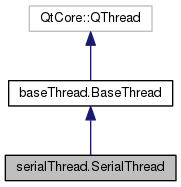
\includegraphics[width=208pt]{classserial_thread_1_1_serial_thread__inherit__graph}
\end{center}
\end{figure}


Collaboration diagram for serial\-Thread.\-Serial\-Thread\-:\nopagebreak
\begin{figure}[H]
\begin{center}
\leavevmode
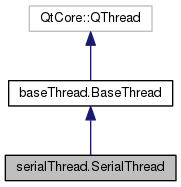
\includegraphics[width=208pt]{classserial_thread_1_1_serial_thread__coll__graph}
\end{center}
\end{figure}
\subsubsection*{Public Member Functions}
\begin{DoxyCompactItemize}
\item 
def \hyperlink{classserial_thread_1_1_serial_thread_a874fcf63db303c69c887b2703d3d1660}{\-\_\-\-\_\-init\-\_\-\-\_\-}
\begin{DoxyCompactList}\small\item\em Constructor. \end{DoxyCompactList}\item 
def \hyperlink{classserial_thread_1_1_serial_thread_abdd58ace4dd79db7f66d15070b2bab5d}{open\-Port}
\begin{DoxyCompactList}\small\item\em Open the defined point. \end{DoxyCompactList}\item 
def \hyperlink{classserial_thread_1_1_serial_thread_a0a71cf4401bb05dbca2b5bf907a22ef2}{run}
\begin{DoxyCompactList}\small\item\em The thread process itself. \end{DoxyCompactList}\item 
def \hyperlink{classserial_thread_1_1_serial_thread_acb2921ccd41a8f36c6503cd996e6e779}{close\-Port}
\begin{DoxyCompactList}\small\item\em Closes the self.\-serial port and waits for the thread to stop. \end{DoxyCompactList}\item 
\hypertarget{classserial_thread_1_1_serial_thread_a7eeeb62dfd322b82e45bac063c895224}{def {\bfseries get\-Acceleration}}\label{classserial_thread_1_1_serial_thread_a7eeeb62dfd322b82e45bac063c895224}

\item 
\hypertarget{classserial_thread_1_1_serial_thread_a1ca654be4f1379aa946c0b523c50ff20}{def {\bfseries get\-Linear\-Accel}}\label{classserial_thread_1_1_serial_thread_a1ca654be4f1379aa946c0b523c50ff20}

\item 
\hypertarget{classserial_thread_1_1_serial_thread_aeab53c96eb90620f814bd189e39a6f52}{def {\bfseries get\-Gyroscope}}\label{classserial_thread_1_1_serial_thread_aeab53c96eb90620f814bd189e39a6f52}

\item 
\hypertarget{classserial_thread_1_1_serial_thread_a9a1638fb77d452d04204e745f20a5436}{def {\bfseries get\-Magnetometer}}\label{classserial_thread_1_1_serial_thread_a9a1638fb77d452d04204e745f20a5436}

\item 
\hypertarget{classserial_thread_1_1_serial_thread_ad47958ff326b2ae20e424141ab55b7f8}{def {\bfseries get\-Euler\-D\-M\-P}}\label{classserial_thread_1_1_serial_thread_ad47958ff326b2ae20e424141ab55b7f8}

\item 
\hypertarget{classserial_thread_1_1_serial_thread_acf4c5d65ee55f42ee3bb85f6437f9652}{def {\bfseries get\-Euler}}\label{classserial_thread_1_1_serial_thread_acf4c5d65ee55f42ee3bb85f6437f9652}

\end{DoxyCompactItemize}
\subsubsection*{Public Attributes}
\begin{DoxyCompactItemize}
\item 
\hypertarget{classserial_thread_1_1_serial_thread_aa8f75dc7fe6b336b0b59c22e691ac333}{{\bfseries imu}}\label{classserial_thread_1_1_serial_thread_aa8f75dc7fe6b336b0b59c22e691ac333}

\item 
\hypertarget{classserial_thread_1_1_serial_thread_af424d14c93b08afa7abb34af4d4a7eb0}{{\bfseries csv\-Scale}}\label{classserial_thread_1_1_serial_thread_af424d14c93b08afa7abb34af4d4a7eb0}

\item 
\hypertarget{classserial_thread_1_1_serial_thread_a1f1509d5fc5fe03dc483fce79ba950de}{{\bfseries csv\-Size}}\label{classserial_thread_1_1_serial_thread_a1f1509d5fc5fe03dc483fce79ba950de}

\item 
\hypertarget{classserial_thread_1_1_serial_thread_adeca93deffc28edc3e087ae387c9d96e}{{\bfseries range\-\_\-accel}}\label{classserial_thread_1_1_serial_thread_adeca93deffc28edc3e087ae387c9d96e}

\item 
\hypertarget{classserial_thread_1_1_serial_thread_ae122e731a3a22bee37bde1720d8e8658}{{\bfseries range\-\_\-gyro}}\label{classserial_thread_1_1_serial_thread_ae122e731a3a22bee37bde1720d8e8658}

\item 
\hypertarget{classserial_thread_1_1_serial_thread_a9086b225ce03b93603e61e673ada983d}{{\bfseries range\-\_\-mag}}\label{classserial_thread_1_1_serial_thread_a9086b225ce03b93603e61e673ada983d}

\item 
\hypertarget{classserial_thread_1_1_serial_thread_addacce9c1aaf0c32a870a1b72dedf4cb}{{\bfseries range\-\_\-euler}}\label{classserial_thread_1_1_serial_thread_addacce9c1aaf0c32a870a1b72dedf4cb}

\item 
\hypertarget{classserial_thread_1_1_serial_thread_a90535f4e52b2f812e2f1c0f214f1921a}{{\bfseries fusion}}\label{classserial_thread_1_1_serial_thread_a90535f4e52b2f812e2f1c0f214f1921a}

\item 
\hypertarget{classserial_thread_1_1_serial_thread_aa0e5b55e35dcb5201ea925dbf6d5316a}{{\bfseries L\-A}}\label{classserial_thread_1_1_serial_thread_aa0e5b55e35dcb5201ea925dbf6d5316a}

\item 
\hypertarget{classserial_thread_1_1_serial_thread_a61b61591e4b8058b7a0c1f153a14d428}{{\bfseries E}}\label{classserial_thread_1_1_serial_thread_a61b61591e4b8058b7a0c1f153a14d428}

\item 
\hypertarget{classserial_thread_1_1_serial_thread_a19e69442978977aa06adc73c34c85735}{{\bfseries exiting}}\label{classserial_thread_1_1_serial_thread_a19e69442978977aa06adc73c34c85735}

\end{DoxyCompactItemize}
\subsubsection*{Static Public Attributes}
\begin{DoxyCompactItemize}
\item 
\hypertarget{classserial_thread_1_1_serial_thread_a06ac7a5102243ffa10f9538532e17bae}{tuple {\bfseries ser} = serial.\-Serial()}\label{classserial_thread_1_1_serial_thread_a06ac7a5102243ffa10f9538532e17bae}

\item 
\hypertarget{classserial_thread_1_1_serial_thread_ad48ef789ece6f219e6d91bac001175cd}{list {\bfseries A} = \mbox{[}.\-0\mbox{]}}\label{classserial_thread_1_1_serial_thread_ad48ef789ece6f219e6d91bac001175cd}

\item 
\hypertarget{classserial_thread_1_1_serial_thread_a0756a22c1321ea6074fc90a05089b723}{list {\bfseries G} = \mbox{[}.\-0\mbox{]}}\label{classserial_thread_1_1_serial_thread_a0756a22c1321ea6074fc90a05089b723}

\item 
\hypertarget{classserial_thread_1_1_serial_thread_a42982b906b746f2073e20a1f3ab17c27}{list {\bfseries M} = \mbox{[}.\-0\mbox{]}}\label{classserial_thread_1_1_serial_thread_a42982b906b746f2073e20a1f3ab17c27}

\item 
\hypertarget{classserial_thread_1_1_serial_thread_a894033843b422979db145acd9f0a4419}{list {\bfseries E\-\_\-dmp} = \mbox{[}.\-3\mbox{]}}\label{classserial_thread_1_1_serial_thread_a894033843b422979db145acd9f0a4419}

\item 
\hypertarget{classserial_thread_1_1_serial_thread_a2eea73a30e105d2b9f6b93a2a63d2a05}{list {\bfseries E} = \mbox{[}.\-0\mbox{]}}\label{classserial_thread_1_1_serial_thread_a2eea73a30e105d2b9f6b93a2a63d2a05}

\item 
\hypertarget{classserial_thread_1_1_serial_thread_a58eea22751715d16929ac4f1cf771451}{list {\bfseries L\-A} = \mbox{[}.\-0\mbox{]}}\label{classserial_thread_1_1_serial_thread_a58eea22751715d16929ac4f1cf771451}

\end{DoxyCompactItemize}


\subsubsection{Detailed Description}
Obtain and scale serial data in a thread. 

Based on the Base\-Thread methods, enables a Qt4 thread for adquiring data from a serial port, using a Qt4 signal to interrupt Qt4 main thread process. 
\begin{DoxyParams}{Parameters}
{\em Base\-Thread} & Basic class for thread handling \\
\hline
\end{DoxyParams}


\subsubsection{Constructor \& Destructor Documentation}
\hypertarget{classserial_thread_1_1_serial_thread_a874fcf63db303c69c887b2703d3d1660}{\index{serial\-Thread\-::\-Serial\-Thread@{serial\-Thread\-::\-Serial\-Thread}!\-\_\-\-\_\-init\-\_\-\-\_\-@{\-\_\-\-\_\-init\-\_\-\-\_\-}}
\index{\-\_\-\-\_\-init\-\_\-\-\_\-@{\-\_\-\-\_\-init\-\_\-\-\_\-}!serialThread::SerialThread@{serial\-Thread\-::\-Serial\-Thread}}
\paragraph[{\-\_\-\-\_\-init\-\_\-\-\_\-}]{\setlength{\rightskip}{0pt plus 5cm}def serial\-Thread.\-Serial\-Thread.\-\_\-\-\_\-init\-\_\-\-\_\- (
\begin{DoxyParamCaption}
\item[{}]{self, }
\item[{}]{device = {\ttfamily 'MPU-\/9150'}}
\end{DoxyParamCaption}
)}}\label{classserial_thread_1_1_serial_thread_a874fcf63db303c69c887b2703d3d1660}


Constructor. 

Enables the basic thread functions and logs 
\begin{DoxyParams}{Parameters}
{\em self} & The object pointer \\
\hline
\end{DoxyParams}


\subsubsection{Member Function Documentation}
\hypertarget{classserial_thread_1_1_serial_thread_acb2921ccd41a8f36c6503cd996e6e779}{\index{serial\-Thread\-::\-Serial\-Thread@{serial\-Thread\-::\-Serial\-Thread}!close\-Port@{close\-Port}}
\index{close\-Port@{close\-Port}!serialThread::SerialThread@{serial\-Thread\-::\-Serial\-Thread}}
\paragraph[{close\-Port}]{\setlength{\rightskip}{0pt plus 5cm}def serial\-Thread.\-Serial\-Thread.\-close\-Port (
\begin{DoxyParamCaption}
\item[{}]{self}
\end{DoxyParamCaption}
)}}\label{classserial_thread_1_1_serial_thread_acb2921ccd41a8f36c6503cd996e6e779}


Closes the self.\-serial port and waits for the thread to stop. 


\begin{DoxyParams}{Parameters}
{\em self} & The objet pointer\# \\
\hline
\end{DoxyParams}
\hypertarget{classserial_thread_1_1_serial_thread_abdd58ace4dd79db7f66d15070b2bab5d}{\index{serial\-Thread\-::\-Serial\-Thread@{serial\-Thread\-::\-Serial\-Thread}!open\-Port@{open\-Port}}
\index{open\-Port@{open\-Port}!serialThread::SerialThread@{serial\-Thread\-::\-Serial\-Thread}}
\paragraph[{open\-Port}]{\setlength{\rightskip}{0pt plus 5cm}def serial\-Thread.\-Serial\-Thread.\-open\-Port (
\begin{DoxyParamCaption}
\item[{}]{self, }
\item[{}]{port = {\ttfamily '/dev/ttyUSB0'}, }
\item[{}]{baud = {\ttfamily 115200}}
\end{DoxyParamCaption}
)}}\label{classserial_thread_1_1_serial_thread_abdd58ace4dd79db7f66d15070b2bab5d}


Open the defined point. 

Configures the serial port, address and speed, and verifies correct initialization and status 
\begin{DoxyParams}{Parameters}
{\em self} & The object pointer \\
\hline
\end{DoxyParams}
\hypertarget{classserial_thread_1_1_serial_thread_a0a71cf4401bb05dbca2b5bf907a22ef2}{\index{serial\-Thread\-::\-Serial\-Thread@{serial\-Thread\-::\-Serial\-Thread}!run@{run}}
\index{run@{run}!serialThread::SerialThread@{serial\-Thread\-::\-Serial\-Thread}}
\paragraph[{run}]{\setlength{\rightskip}{0pt plus 5cm}def serial\-Thread.\-Serial\-Thread.\-run (
\begin{DoxyParamCaption}
\item[{}]{self}
\end{DoxyParamCaption}
)}}\label{classserial_thread_1_1_serial_thread_a0a71cf4401bb05dbca2b5bf907a22ef2}


The thread process itself. 

Defines the \char`\"{}loop\char`\"{} method of the thread
\begin{DoxyItemize}
\item Obtain self.\-data from the defined self.\-serial port
\item Separate in C\-S\-V format
\item Assuming the input from a M\-P\-U-\/9150, scales self.\-data
\item Manage incorrect C\-S\-V format (by size)
\item Manage incomplete self.\-data transfer
\item Notify main thread (Qt4) with a signal 
\begin{DoxyParams}{Parameters}
{\em self} & The objetc pointer \\
\hline
\end{DoxyParams}

\end{DoxyItemize}

The documentation for this class was generated from the following file\-:\begin{DoxyCompactItemize}
\item 
I\-M\-U\-Graph/serial\-Thread.\-py\end{DoxyCompactItemize}

\hypertarget{classserial_thread__mutiprocessing_1_1_serial_thread}{\subsection{serial\-Thread\-\_\-mutiprocessing.\-Serial\-Thread Class Reference}
\label{classserial_thread__mutiprocessing_1_1_serial_thread}\index{serial\-Thread\-\_\-mutiprocessing.\-Serial\-Thread@{serial\-Thread\-\_\-mutiprocessing.\-Serial\-Thread}}
}


Obtain and scale serial data in a thread.  




Inheritance diagram for serial\-Thread\-\_\-mutiprocessing.\-Serial\-Thread\-:\nopagebreak
\begin{figure}[H]
\begin{center}
\leavevmode
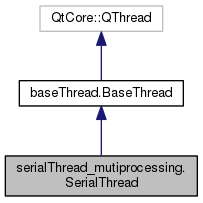
\includegraphics[width=224pt]{classserial_thread__mutiprocessing_1_1_serial_thread__inherit__graph}
\end{center}
\end{figure}


Collaboration diagram for serial\-Thread\-\_\-mutiprocessing.\-Serial\-Thread\-:\nopagebreak
\begin{figure}[H]
\begin{center}
\leavevmode
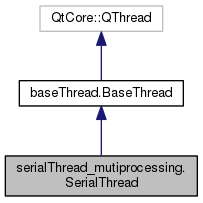
\includegraphics[width=224pt]{classserial_thread__mutiprocessing_1_1_serial_thread__coll__graph}
\end{center}
\end{figure}
\subsubsection*{Public Member Functions}
\begin{DoxyCompactItemize}
\item 
def \hyperlink{classserial_thread__mutiprocessing_1_1_serial_thread_a1e8d9f128a8591dc91bc14e2e3dfea40}{\-\_\-\-\_\-init\-\_\-\-\_\-}
\begin{DoxyCompactList}\small\item\em Constructor. \end{DoxyCompactList}\item 
def \hyperlink{classserial_thread__mutiprocessing_1_1_serial_thread_a49c1452622fb407aef0f413c5cab3099}{open\-Port}
\begin{DoxyCompactList}\small\item\em Open the defined point. \end{DoxyCompactList}\item 
def \hyperlink{classserial_thread__mutiprocessing_1_1_serial_thread_aa4ea3b84bdda2e44d009d19ac2f0ab88}{run}
\begin{DoxyCompactList}\small\item\em The thread process itself. \end{DoxyCompactList}\item 
def \hyperlink{classserial_thread__mutiprocessing_1_1_serial_thread_af1dcde994351eb5cf14d9232537481b9}{close\-Port}
\begin{DoxyCompactList}\small\item\em Closes the self.\-serial port and waits for the thread to stop. \end{DoxyCompactList}\item 
\hypertarget{classserial_thread__mutiprocessing_1_1_serial_thread_a21d756af58ff7307c11f4bd561466334}{def {\bfseries get\-Acceleration}}\label{classserial_thread__mutiprocessing_1_1_serial_thread_a21d756af58ff7307c11f4bd561466334}

\item 
\hypertarget{classserial_thread__mutiprocessing_1_1_serial_thread_aba2db486301fefccdae03ae340929e8f}{def {\bfseries get\-Linear\-Accel}}\label{classserial_thread__mutiprocessing_1_1_serial_thread_aba2db486301fefccdae03ae340929e8f}

\item 
\hypertarget{classserial_thread__mutiprocessing_1_1_serial_thread_aae16862501d11804556514c61000b7ca}{def {\bfseries get\-Gyroscope}}\label{classserial_thread__mutiprocessing_1_1_serial_thread_aae16862501d11804556514c61000b7ca}

\item 
\hypertarget{classserial_thread__mutiprocessing_1_1_serial_thread_a0b2b452f46787771159cf822cbc91328}{def {\bfseries get\-Magnetometer}}\label{classserial_thread__mutiprocessing_1_1_serial_thread_a0b2b452f46787771159cf822cbc91328}

\item 
\hypertarget{classserial_thread__mutiprocessing_1_1_serial_thread_a13c28f06f370a22b23116d8cdef03a71}{def {\bfseries get\-Euler\-D\-M\-P}}\label{classserial_thread__mutiprocessing_1_1_serial_thread_a13c28f06f370a22b23116d8cdef03a71}

\item 
\hypertarget{classserial_thread__mutiprocessing_1_1_serial_thread_af1075662e8123728f5dd9379445ed5bd}{def {\bfseries get\-Euler}}\label{classserial_thread__mutiprocessing_1_1_serial_thread_af1075662e8123728f5dd9379445ed5bd}

\end{DoxyCompactItemize}
\subsubsection*{Public Attributes}
\begin{DoxyCompactItemize}
\item 
\hypertarget{classserial_thread__mutiprocessing_1_1_serial_thread_ad4920675cfd07a9bb791aa7110189987}{{\bfseries imu}}\label{classserial_thread__mutiprocessing_1_1_serial_thread_ad4920675cfd07a9bb791aa7110189987}

\item 
\hypertarget{classserial_thread__mutiprocessing_1_1_serial_thread_a909c0614f0634d4e4a3c9d367e31b6f5}{{\bfseries csv\-Scale}}\label{classserial_thread__mutiprocessing_1_1_serial_thread_a909c0614f0634d4e4a3c9d367e31b6f5}

\item 
\hypertarget{classserial_thread__mutiprocessing_1_1_serial_thread_a76065582070409642b4504e5418743cc}{{\bfseries csv\-Size}}\label{classserial_thread__mutiprocessing_1_1_serial_thread_a76065582070409642b4504e5418743cc}

\item 
\hypertarget{classserial_thread__mutiprocessing_1_1_serial_thread_aa623f355a6f9add29fd1c8e52ab7746f}{{\bfseries range\-\_\-accel}}\label{classserial_thread__mutiprocessing_1_1_serial_thread_aa623f355a6f9add29fd1c8e52ab7746f}

\item 
\hypertarget{classserial_thread__mutiprocessing_1_1_serial_thread_a0e885ee8b00b2df25e341b40046edbc1}{{\bfseries range\-\_\-gyro}}\label{classserial_thread__mutiprocessing_1_1_serial_thread_a0e885ee8b00b2df25e341b40046edbc1}

\item 
\hypertarget{classserial_thread__mutiprocessing_1_1_serial_thread_adbd83fe021f73d343c4b34bdb584b364}{{\bfseries range\-\_\-mag}}\label{classserial_thread__mutiprocessing_1_1_serial_thread_adbd83fe021f73d343c4b34bdb584b364}

\item 
\hypertarget{classserial_thread__mutiprocessing_1_1_serial_thread_aeec7d887f15934388b08fb6358e7ab4e}{{\bfseries range\-\_\-euler}}\label{classserial_thread__mutiprocessing_1_1_serial_thread_aeec7d887f15934388b08fb6358e7ab4e}

\item 
\hypertarget{classserial_thread__mutiprocessing_1_1_serial_thread_aaa4a858bca292ee3e14bc893d2365ded}{{\bfseries fusion}}\label{classserial_thread__mutiprocessing_1_1_serial_thread_aaa4a858bca292ee3e14bc893d2365ded}

\item 
\hypertarget{classserial_thread__mutiprocessing_1_1_serial_thread_a2e780aa8d9d4116608af64a3d5348ec3}{{\bfseries L\-A}}\label{classserial_thread__mutiprocessing_1_1_serial_thread_a2e780aa8d9d4116608af64a3d5348ec3}

\item 
\hypertarget{classserial_thread__mutiprocessing_1_1_serial_thread_a0b1b5c0a51a56c846d74039208a3d56f}{{\bfseries E}}\label{classserial_thread__mutiprocessing_1_1_serial_thread_a0b1b5c0a51a56c846d74039208a3d56f}

\item 
\hypertarget{classserial_thread__mutiprocessing_1_1_serial_thread_a6bbaa87b5c983fd8de8ea625b6b81647}{{\bfseries exiting}}\label{classserial_thread__mutiprocessing_1_1_serial_thread_a6bbaa87b5c983fd8de8ea625b6b81647}

\end{DoxyCompactItemize}
\subsubsection*{Static Public Attributes}
\begin{DoxyCompactItemize}
\item 
\hypertarget{classserial_thread__mutiprocessing_1_1_serial_thread_a53f65d82752759b57636d036b8a39ac7}{tuple {\bfseries ser} = serial.\-Serial()}\label{classserial_thread__mutiprocessing_1_1_serial_thread_a53f65d82752759b57636d036b8a39ac7}

\item 
\hypertarget{classserial_thread__mutiprocessing_1_1_serial_thread_a43b0c4ff6a34de602ccf7194bc8085ab}{list {\bfseries A} = \mbox{[}.\-0\mbox{]}}\label{classserial_thread__mutiprocessing_1_1_serial_thread_a43b0c4ff6a34de602ccf7194bc8085ab}

\item 
\hypertarget{classserial_thread__mutiprocessing_1_1_serial_thread_a5ac3a71646a9a65fd5744968006e232e}{list {\bfseries G} = \mbox{[}.\-0\mbox{]}}\label{classserial_thread__mutiprocessing_1_1_serial_thread_a5ac3a71646a9a65fd5744968006e232e}

\item 
\hypertarget{classserial_thread__mutiprocessing_1_1_serial_thread_a8e820bcb387f80388a6957a046695cd5}{list {\bfseries M} = \mbox{[}.\-0\mbox{]}}\label{classserial_thread__mutiprocessing_1_1_serial_thread_a8e820bcb387f80388a6957a046695cd5}

\item 
\hypertarget{classserial_thread__mutiprocessing_1_1_serial_thread_a44901b90485df32694098955ecf88124}{list {\bfseries E\-\_\-dmp} = \mbox{[}.\-3\mbox{]}}\label{classserial_thread__mutiprocessing_1_1_serial_thread_a44901b90485df32694098955ecf88124}

\item 
\hypertarget{classserial_thread__mutiprocessing_1_1_serial_thread_a3199e8aac32a2614df984ab94702cb84}{list {\bfseries E} = \mbox{[}.\-0\mbox{]}}\label{classserial_thread__mutiprocessing_1_1_serial_thread_a3199e8aac32a2614df984ab94702cb84}

\item 
\hypertarget{classserial_thread__mutiprocessing_1_1_serial_thread_a65fc676fc0c37ad5b5c4c8643f63e2ae}{list {\bfseries L\-A} = \mbox{[}.\-0\mbox{]}}\label{classserial_thread__mutiprocessing_1_1_serial_thread_a65fc676fc0c37ad5b5c4c8643f63e2ae}

\end{DoxyCompactItemize}


\subsubsection{Detailed Description}
Obtain and scale serial data in a thread. 

Based on the Base\-Thread methods, enables a Qt4 thread for adquiring data from a serial port, using a Qt4 signal to interrupt Qt4 main thread process. 
\begin{DoxyParams}{Parameters}
{\em Base\-Thread} & Basic class for thread handling \\
\hline
\end{DoxyParams}


\subsubsection{Constructor \& Destructor Documentation}
\hypertarget{classserial_thread__mutiprocessing_1_1_serial_thread_a1e8d9f128a8591dc91bc14e2e3dfea40}{\index{serial\-Thread\-\_\-mutiprocessing\-::\-Serial\-Thread@{serial\-Thread\-\_\-mutiprocessing\-::\-Serial\-Thread}!\-\_\-\-\_\-init\-\_\-\-\_\-@{\-\_\-\-\_\-init\-\_\-\-\_\-}}
\index{\-\_\-\-\_\-init\-\_\-\-\_\-@{\-\_\-\-\_\-init\-\_\-\-\_\-}!serialThread_mutiprocessing::SerialThread@{serial\-Thread\-\_\-mutiprocessing\-::\-Serial\-Thread}}
\paragraph[{\-\_\-\-\_\-init\-\_\-\-\_\-}]{\setlength{\rightskip}{0pt plus 5cm}def serial\-Thread\-\_\-mutiprocessing.\-Serial\-Thread.\-\_\-\-\_\-init\-\_\-\-\_\- (
\begin{DoxyParamCaption}
\item[{}]{self, }
\item[{}]{device = {\ttfamily 'MPU-\/9150'}}
\end{DoxyParamCaption}
)}}\label{classserial_thread__mutiprocessing_1_1_serial_thread_a1e8d9f128a8591dc91bc14e2e3dfea40}


Constructor. 

Enables the basic thread functions and logs 
\begin{DoxyParams}{Parameters}
{\em self} & The object pointer \\
\hline
\end{DoxyParams}


\subsubsection{Member Function Documentation}
\hypertarget{classserial_thread__mutiprocessing_1_1_serial_thread_af1dcde994351eb5cf14d9232537481b9}{\index{serial\-Thread\-\_\-mutiprocessing\-::\-Serial\-Thread@{serial\-Thread\-\_\-mutiprocessing\-::\-Serial\-Thread}!close\-Port@{close\-Port}}
\index{close\-Port@{close\-Port}!serialThread_mutiprocessing::SerialThread@{serial\-Thread\-\_\-mutiprocessing\-::\-Serial\-Thread}}
\paragraph[{close\-Port}]{\setlength{\rightskip}{0pt plus 5cm}def serial\-Thread\-\_\-mutiprocessing.\-Serial\-Thread.\-close\-Port (
\begin{DoxyParamCaption}
\item[{}]{self}
\end{DoxyParamCaption}
)}}\label{classserial_thread__mutiprocessing_1_1_serial_thread_af1dcde994351eb5cf14d9232537481b9}


Closes the self.\-serial port and waits for the thread to stop. 


\begin{DoxyParams}{Parameters}
{\em self} & The objet pointer\# \\
\hline
\end{DoxyParams}
\hypertarget{classserial_thread__mutiprocessing_1_1_serial_thread_a49c1452622fb407aef0f413c5cab3099}{\index{serial\-Thread\-\_\-mutiprocessing\-::\-Serial\-Thread@{serial\-Thread\-\_\-mutiprocessing\-::\-Serial\-Thread}!open\-Port@{open\-Port}}
\index{open\-Port@{open\-Port}!serialThread_mutiprocessing::SerialThread@{serial\-Thread\-\_\-mutiprocessing\-::\-Serial\-Thread}}
\paragraph[{open\-Port}]{\setlength{\rightskip}{0pt plus 5cm}def serial\-Thread\-\_\-mutiprocessing.\-Serial\-Thread.\-open\-Port (
\begin{DoxyParamCaption}
\item[{}]{self, }
\item[{}]{port = {\ttfamily '/dev/ttyUSB0'}, }
\item[{}]{baud = {\ttfamily 115200}}
\end{DoxyParamCaption}
)}}\label{classserial_thread__mutiprocessing_1_1_serial_thread_a49c1452622fb407aef0f413c5cab3099}


Open the defined point. 

Configures the serial port, address and speed, and verifies correct initialization and status 
\begin{DoxyParams}{Parameters}
{\em self} & The object pointer \\
\hline
\end{DoxyParams}
\hypertarget{classserial_thread__mutiprocessing_1_1_serial_thread_aa4ea3b84bdda2e44d009d19ac2f0ab88}{\index{serial\-Thread\-\_\-mutiprocessing\-::\-Serial\-Thread@{serial\-Thread\-\_\-mutiprocessing\-::\-Serial\-Thread}!run@{run}}
\index{run@{run}!serialThread_mutiprocessing::SerialThread@{serial\-Thread\-\_\-mutiprocessing\-::\-Serial\-Thread}}
\paragraph[{run}]{\setlength{\rightskip}{0pt plus 5cm}def serial\-Thread\-\_\-mutiprocessing.\-Serial\-Thread.\-run (
\begin{DoxyParamCaption}
\item[{}]{self}
\end{DoxyParamCaption}
)}}\label{classserial_thread__mutiprocessing_1_1_serial_thread_aa4ea3b84bdda2e44d009d19ac2f0ab88}


The thread process itself. 

Defines the \char`\"{}loop\char`\"{} method of the thread
\begin{DoxyItemize}
\item Obtain self.\-data from the defined self.\-serial port
\item Separate in C\-S\-V format
\item Assuming the input from a M\-P\-U-\/9150, scales self.\-data
\item Manage incorrect C\-S\-V format (by size)
\item Manage incomplete self.\-data transfer
\item Notify main thread (Qt4) with a signal 
\begin{DoxyParams}{Parameters}
{\em self} & The objetc pointer \\
\hline
\end{DoxyParams}

\end{DoxyItemize}

The documentation for this class was generated from the following file\-:\begin{DoxyCompactItemize}
\item 
I\-M\-U\-Graph/serial\-Thread\-\_\-mutiprocessing.\-py\end{DoxyCompactItemize}

\hypertarget{classgui_1_1_ui___main_window}{\subsection{gui.\-Ui\-\_\-\-Main\-Window Class Reference}
\label{classgui_1_1_ui___main_window}\index{gui.\-Ui\-\_\-\-Main\-Window@{gui.\-Ui\-\_\-\-Main\-Window}}
}


Inheritance diagram for gui.\-Ui\-\_\-\-Main\-Window\-:\nopagebreak
\begin{figure}[H]
\begin{center}
\leavevmode
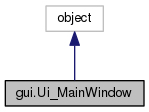
\includegraphics[width=184pt]{classgui_1_1_ui___main_window__inherit__graph}
\end{center}
\end{figure}


Collaboration diagram for gui.\-Ui\-\_\-\-Main\-Window\-:\nopagebreak
\begin{figure}[H]
\begin{center}
\leavevmode
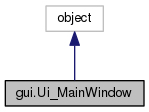
\includegraphics[width=184pt]{classgui_1_1_ui___main_window__coll__graph}
\end{center}
\end{figure}
\subsubsection*{Public Member Functions}
\begin{DoxyCompactItemize}
\item 
\hypertarget{classgui_1_1_ui___main_window_a9a1bbcec1be5acbadaf4bbe2cb00ac67}{def {\bfseries setup\-Ui}}\label{classgui_1_1_ui___main_window_a9a1bbcec1be5acbadaf4bbe2cb00ac67}

\item 
\hypertarget{classgui_1_1_ui___main_window_acf875fda63898e38deac938fcaac6b89}{def {\bfseries retranslate\-Ui}}\label{classgui_1_1_ui___main_window_acf875fda63898e38deac938fcaac6b89}

\end{DoxyCompactItemize}
\subsubsection*{Public Attributes}
\begin{DoxyCompactItemize}
\item 
\hypertarget{classgui_1_1_ui___main_window_ac900ad92ffecd9461283d42ed0bdb934}{{\bfseries centralwidget}}\label{classgui_1_1_ui___main_window_ac900ad92ffecd9461283d42ed0bdb934}

\item 
\hypertarget{classgui_1_1_ui___main_window_a75f1821f02dfd198b796a50a2d811f76}{{\bfseries grid\-Layout}}\label{classgui_1_1_ui___main_window_a75f1821f02dfd198b796a50a2d811f76}

\item 
\hypertarget{classgui_1_1_ui___main_window_a8d1b5d256b6d05fb285d543c2a759a06}{{\bfseries c\-Box\-\_\-\-Speed}}\label{classgui_1_1_ui___main_window_a8d1b5d256b6d05fb285d543c2a759a06}

\item 
\hypertarget{classgui_1_1_ui___main_window_aa88b414e1f81f2211401870bbaf2db97}{{\bfseries p\-Button\-\_\-\-Stop}}\label{classgui_1_1_ui___main_window_aa88b414e1f81f2211401870bbaf2db97}

\item 
\hypertarget{classgui_1_1_ui___main_window_acdf0c1ec4fb0daaa5c4b635239ddf9ae}{{\bfseries c\-Box\-\_\-\-Port}}\label{classgui_1_1_ui___main_window_acdf0c1ec4fb0daaa5c4b635239ddf9ae}

\item 
\hypertarget{classgui_1_1_ui___main_window_a44a88eaa0c3162b45e5f8151ca13ca52}{{\bfseries plt1}}\label{classgui_1_1_ui___main_window_a44a88eaa0c3162b45e5f8151ca13ca52}

\item 
\hypertarget{classgui_1_1_ui___main_window_afba40446e19abbd702c0a47f3668a141}{{\bfseries plt5}}\label{classgui_1_1_ui___main_window_afba40446e19abbd702c0a47f3668a141}

\item 
\hypertarget{classgui_1_1_ui___main_window_a5eed648bb2eaa08d8ef42bff16ab189c}{{\bfseries plt4}}\label{classgui_1_1_ui___main_window_a5eed648bb2eaa08d8ef42bff16ab189c}

\item 
\hypertarget{classgui_1_1_ui___main_window_abd1829eef2159f439ee90b3967fc88dd}{{\bfseries plt2}}\label{classgui_1_1_ui___main_window_abd1829eef2159f439ee90b3967fc88dd}

\item 
\hypertarget{classgui_1_1_ui___main_window_a13aa9dcb55514e5b0f4905bb4b1c6493}{{\bfseries p\-Button\-\_\-\-Start}}\label{classgui_1_1_ui___main_window_a13aa9dcb55514e5b0f4905bb4b1c6493}

\item 
\hypertarget{classgui_1_1_ui___main_window_a2fd8b037a76faf4abd06ea4529723ea3}{{\bfseries plt3}}\label{classgui_1_1_ui___main_window_a2fd8b037a76faf4abd06ea4529723ea3}

\item 
\hypertarget{classgui_1_1_ui___main_window_ac19287cfecfb2ced23d8410b38593507}{{\bfseries plt6}}\label{classgui_1_1_ui___main_window_ac19287cfecfb2ced23d8410b38593507}

\item 
\hypertarget{classgui_1_1_ui___main_window_ae581f538f6927354dcac66d736892953}{{\bfseries p\-Button\-\_\-\-Cube}}\label{classgui_1_1_ui___main_window_ae581f538f6927354dcac66d736892953}

\item 
\hypertarget{classgui_1_1_ui___main_window_ad9e33d07818247968967ffae81dfd588}{{\bfseries ch\-Box\-\_\-export}}\label{classgui_1_1_ui___main_window_ad9e33d07818247968967ffae81dfd588}

\item 
\hypertarget{classgui_1_1_ui___main_window_aa68232933c2104617d7e7f9ade44946b}{{\bfseries c\-Box\-\_\-\-I\-M\-U}}\label{classgui_1_1_ui___main_window_aa68232933c2104617d7e7f9ade44946b}

\item 
\hypertarget{classgui_1_1_ui___main_window_a146d1c780e596fb732fe26f890da62ea}{{\bfseries p\-Button\-\_\-\-Reset}}\label{classgui_1_1_ui___main_window_a146d1c780e596fb732fe26f890da62ea}

\item 
\hypertarget{classgui_1_1_ui___main_window_a7a1c098550ce150f46c3532b3f84a931}{{\bfseries statusbar}}\label{classgui_1_1_ui___main_window_a7a1c098550ce150f46c3532b3f84a931}

\item 
\hypertarget{classgui_1_1_ui___main_window_a569cc7e806577657e55ac9eb75edd60e}{{\bfseries menubar}}\label{classgui_1_1_ui___main_window_a569cc7e806577657e55ac9eb75edd60e}

\item 
\hypertarget{classgui_1_1_ui___main_window_acd8285bf72ef72bb25bb4d23929f19a7}{{\bfseries menu\-File}}\label{classgui_1_1_ui___main_window_acd8285bf72ef72bb25bb4d23929f19a7}

\item 
\hypertarget{classgui_1_1_ui___main_window_a194ed355e510756cb9f735aa07c94fe9}{{\bfseries action\-Linear\-\_\-\-Acceleration}}\label{classgui_1_1_ui___main_window_a194ed355e510756cb9f735aa07c94fe9}

\item 
\hypertarget{classgui_1_1_ui___main_window_ac7be810d7eff8c487e35f24f6871940d}{{\bfseries action\-Euler\-\_\-\-Rotation}}\label{classgui_1_1_ui___main_window_ac7be810d7eff8c487e35f24f6871940d}

\item 
\hypertarget{classgui_1_1_ui___main_window_a356c581991692e840734d9dc85a54f47}{{\bfseries action\-Linear\-\_\-\-Acceleration\-\_\-2}}\label{classgui_1_1_ui___main_window_a356c581991692e840734d9dc85a54f47}

\item 
\hypertarget{classgui_1_1_ui___main_window_a72445113fdb988573ed62663299262ab}{{\bfseries action\-G\-\_\-force}}\label{classgui_1_1_ui___main_window_a72445113fdb988573ed62663299262ab}

\item 
\hypertarget{classgui_1_1_ui___main_window_aae9432d44e60809aa10c1782eee6d155}{{\bfseries action\-Meters\-\_\-seg\-\_\-2}}\label{classgui_1_1_ui___main_window_aae9432d44e60809aa10c1782eee6d155}

\item 
\hypertarget{classgui_1_1_ui___main_window_a760a126ef8f76ff5fcf3c0c09d61a951}{{\bfseries action\-Rad\-\_\-seg}}\label{classgui_1_1_ui___main_window_a760a126ef8f76ff5fcf3c0c09d61a951}

\item 
\hypertarget{classgui_1_1_ui___main_window_a5a1a24a90b150d188a3bba43c31f2884}{{\bfseries action\-Deg\-\_\-seg}}\label{classgui_1_1_ui___main_window_a5a1a24a90b150d188a3bba43c31f2884}

\item 
\hypertarget{classgui_1_1_ui___main_window_a50c3bb05de615e54db162cb54107a092}{{\bfseries action\-Yawn\-\_\-\-Pitch\-\_\-\-Roll}}\label{classgui_1_1_ui___main_window_a50c3bb05de615e54db162cb54107a092}

\item 
\hypertarget{classgui_1_1_ui___main_window_a0573105f763807eef541b4de4be1d3e1}{{\bfseries action\-Euler\-\_\-\-Angles}}\label{classgui_1_1_ui___main_window_a0573105f763807eef541b4de4be1d3e1}

\item 
\hypertarget{classgui_1_1_ui___main_window_adfdd860edfc5ae4a29ca3ae5d135b824}{{\bfseries action\-Scan\-\_\-\-Serial\-\_\-ports}}\label{classgui_1_1_ui___main_window_adfdd860edfc5ae4a29ca3ae5d135b824}

\end{DoxyCompactItemize}


The documentation for this class was generated from the following file\-:\begin{DoxyCompactItemize}
\item 
I\-M\-U\-Graph/gui.\-py\end{DoxyCompactItemize}

%--- End generated contents ---

% Index
\newpage
\phantomsection
\addcontentsline{toc}{section}{Index}
\printindex

\end{document}
